% This is Lecture Notes for PET504E Advanced Well Test Analysis
%
\documentclass{llncs}

\usepackage{graphicx}
\usepackage{framed,color}
\definecolor{shadecolor}{rgb}{0.3921,0.58431,0.9294}
\usepackage{llncsdoc}
\usepackage{savesym}
\usepackage{float}
\savesymbol{note}
\usepackage{color} % Allow text colors
\usepackage{enumerate}
\usepackage{amsmath}

%\usepackage{fullpage}
\usepackage[finalnew]{trackchanges}
%\usepackage[finalold]{trackchanges}
%\usepackage[footnotes]{trackchanges}
%\usepackage[inline]{trackchanges}
%\usepackage[margins]{trackchanges}
%\usepackage[margins, movemargins]{trackchanges}
%\usepackage[margins, adjustmargins]{trackchanges}
%
\addeditor{Murat \c{C}{\i}nar}
\addeditor{Mustafa Onur}
\restoresymbol{Trck}{note}
 \numberwithin{equation}{section}
 \numberwithin{figure}{section}
 \numberwithin{table}{section}
%
%\usepackage{nomencl}
%\makenomenclature
%
\begin{document}
    \markboth{PET504E Advanced Well Test Analysis}{PET504E Advanced Well Test Analysis}
    \thispagestyle{empty}
    \begin{flushleft}
        \LARGE\bfseries Lecture Notes\\[1cm]
    \end{flushleft}
    \rule{\textwidth}{1pt}
    \vspace{2pt}
    \begin{flushright}
        \Huge
            \begin{tabular}{@{}l}
                PET504E \\
                Advanced Well Test \\
                Analysis\\[6pt]
                {\Large 2012}
            \end{tabular}
        \end{flushright}
    \rule{\textwidth}{1pt}

    \begin{flushleft}
        \LARGE\bfseries by\\ Prof. Dr. Mustafa Onur \\[0.5cm]
        Dr. Murat \c{C}{\i}nar\\

    \end{flushleft}
    \vfill

    \section{Introduction}
%
    The term "Well Testing" \add[Murat \c{C}{\i}nar]{as it} is used in Petroleum Industry means the measuring of a formation's
    (or reservoir's) pressure (and/or rate) response to flow from a well. The term "Well Testing"
    is generally used with the term "Pressure Transient Analysis", interchangeably. It is an indirect
    measurement technique as opposed to direct methods such as fluid sampling or coring. Well testing
    provides dynamic information on the reservoir whereas direct measurements only provide static
    information, which is not sufficient for predicting the behavior of the reservoir.\\

    Simply, the objective of well testing is to deduce quantitative information about the well/reservoir system
    under consideration from its response to a given input. Input (or input signal) is used for perturbing one or more
    wells so that the output (signal) exhibiting the response of the reservoir is obtained at the perturbated well and/or
    adjacent wells. In practice, the input is equivalent to controlling the well behavior \remove[Murat \c{C}{\i}nar]{and} created by changing
    the flow rate or the pressure at the well (Mathematically specifying the well behavior is equivalent to specifying
    a boundary condition). A common example for creating an input signal is \add[Murat \c{C}{\i}nar]{a} build up test
    \change[Murat \c{C}{\i}nar]{in which}{where} we change the rate to zero by shutting-in the well. Reservoir response,
    \remove[Murat \c{C}{\i}nar]{which is} also called output signal, to a given input is monitored by measuring the
    pressure change (or rate change) at the \remove[Murat \c{C}{\i}nar]{same}  well. This process is illustrated as,

    \begin{figure}[h]
        \setlength{\unitlength}{0.14in} % selecting unit length
        \centering % used for centering Figure
        \begin{picture}(32,15) % picture environment with the size (dimensions)
        % 32 length units wide, and 15 units high.
            \put(3,4){\framebox(6,3){Input}}
            \put(13,4){\framebox(6,3){System}}
            \put(23,4){\framebox(6,3){Output}}
            \put(14,3){(Unknown)}
            \put(6,1){I}
            \put(16,1){S}
            \put(26,1){O}
            \put(9,5.5){\vector(1,0){4}}
            \put(19,5.5){\vector(1,0){4}}
            \put(9,1){\vector(1,0){4}}
            \put(19,1){\vector(1,0){4}}
        \end{picture}
        \caption{Block diagram ?????}
        \label{input_output} % label to refer figure in text
    \end{figure}

    Typical examples for input and output signals as used in petroleum industry are shown in Fig. \ref{Transient_phenomena}.
    \begin{figure}
        \begin{center}
        \includegraphics[scale=0.75]{Transient_phenomena.pdf}
        \end{center}
        \caption{Typical input and output signals - Transient phenomena.}
        \label{Transient_phenomena}
    \end{figure}


    From reservoir response as monitored by the "output signal", we would like to determine information related to the followings:
    \begin{itemize}
        \item Fluid in place; pore volume, ${\phi}hA$.
        \item Ability of reservoir to transfer fluid, $kh$ (or transmissibility, $\frac{kh}{\mu}$).
        \item Determination of average reservoir \change[Murat \c{C}{\i}nar]{average}{pressure}, $\overline{P}$, which is the driving force in the reservoir \Trcknote[Murat \c{C}{\i}nar]{Based upon the explanation you gave about the pressure decline recently, I am not sure if this statement is correct.}
        \item Prediction of rate versus time data.
        \item Initial recovery, is the reservoir worth producing.
        \item Is there any damage around the wellbore impeding the flow? skin factor, $s$.
        \item Reservoir description (type of reservoir, flow boundaries (faults)).
        \item Distance to fluid interface \change[Murat \c{C}{\i}nar]{which}{that} is important determining swept zone for secondary and tertiary methods.
    \end{itemize}
    Interpretation of well test data consist of basically three steps:

    \begin{enumerate}[(i)]
        \item Determination of the one most appropriate reservoir / wellbore (mathematical) model \change[Murat \c{C}{\i}nar]{to}{of} the actual system. We also call such a model as the interpretation model. \change[Murat \c{C}{\i}nar]{Here our hope is that the model chosen will produce an output signal to a given input which is as close as possible to that of the actual system.}{Here our intention is to find a representative mathematical model that reproduces, as close as possible, the output of the actual system for a given input.} This is known as the inverse problem. \add[Murat \c{C}{\i}nar]{We are trying to obtain information about the physical system by using observed measurements.} Unfortunately, the solution of inverse problem often yields non-unique results. \change[Murat \c{C}{\i}nar]{With}{By} non-unique results, we mean that several different interpretation models \change[Murat \c{C}{\i}nar]{can}{may} generate an output signal (response) to a given input \change[Murat \c{C}{\i}nar]{which}{that} is similar (or identical) to that of the actual system. The inverse problem can be represented by the following equation.

        \begin{equation}
            \Sigma ={O}/{I}\;\approx S
            \label{InvP}
        \end{equation}

            where $\Sigma$ denotes the interpretation model, $S$ denotes the actual system. In inverse problem, as can be seen from Eq.\ref{InvP}, it may be possible to obtain the same outputs to a given $I$ for different $\Sigma_{i}$'s\change[Murat \c{C}{\i}nar]{. However}{,however}, the number of alternative models (solutions) can be reduced as the number and the range of output signal measurements.\\

        \item Once the appropriate model is determined, estimate the parameters of the actual system $S$. \change[Murat \c{C}{\i}nar]{Such parameters can be}{These parameters are} $kh$, $s$, $\phi$, $C$, $\lambda$, $w$ etc. This is known as \remove[Murat \c{C}{\i}nar]{the}parameter estimation\remove[Murat \c{C}{\i}nar]{problem}\change[Murat \c{C}{\i}nar]{.  It is}{ and} achieved by adjusting the parameters of the model by different \add[Murat \c{C}{\i}nar]{mathematical} methods to obtain an output signal, $\Omega$, that is always qualitatively identical (within some tolerance) to that of \add[Murat \c{C}{\i}nar]{the} actual system, $O$. The computation of $\Omega$ is known as
            the "\change[Murat \c{C}{\i}nar]{direct}{forward} problem" in mathematics. Contrary to the inverse problem, the solution of the \change[Murat \c{C}{\i}nar]{direct}{forward} problem is always unique for a given system; that is,
        \begin{equation}
            I\times \Sigma =\Omega \approx 0
            \label{ForP}
        \end{equation}
            The adjusted parameters of the interpretation model are assumed to represent the parameters of the real system $S$.  \Trcknote[Murat \c{C}{\i}nar]{I think we should discuss this phrase. Does the real system have any parameters? I do not think so... This is something conceptual we need to think about}
        \item Validate the results of the interpretation. This can be achieved by using the parameters determined from part $(ii)$ in the model
              to generate output signals for the entire range of \add[Murat \c{C}{\i}nar]{the} test and by comparing these outputs with the \change[Murat \c{C}{\i}nar]{measured ones}{physical measurements}.
    \end{enumerate}

    \begin{figure}
        \begin{center}
        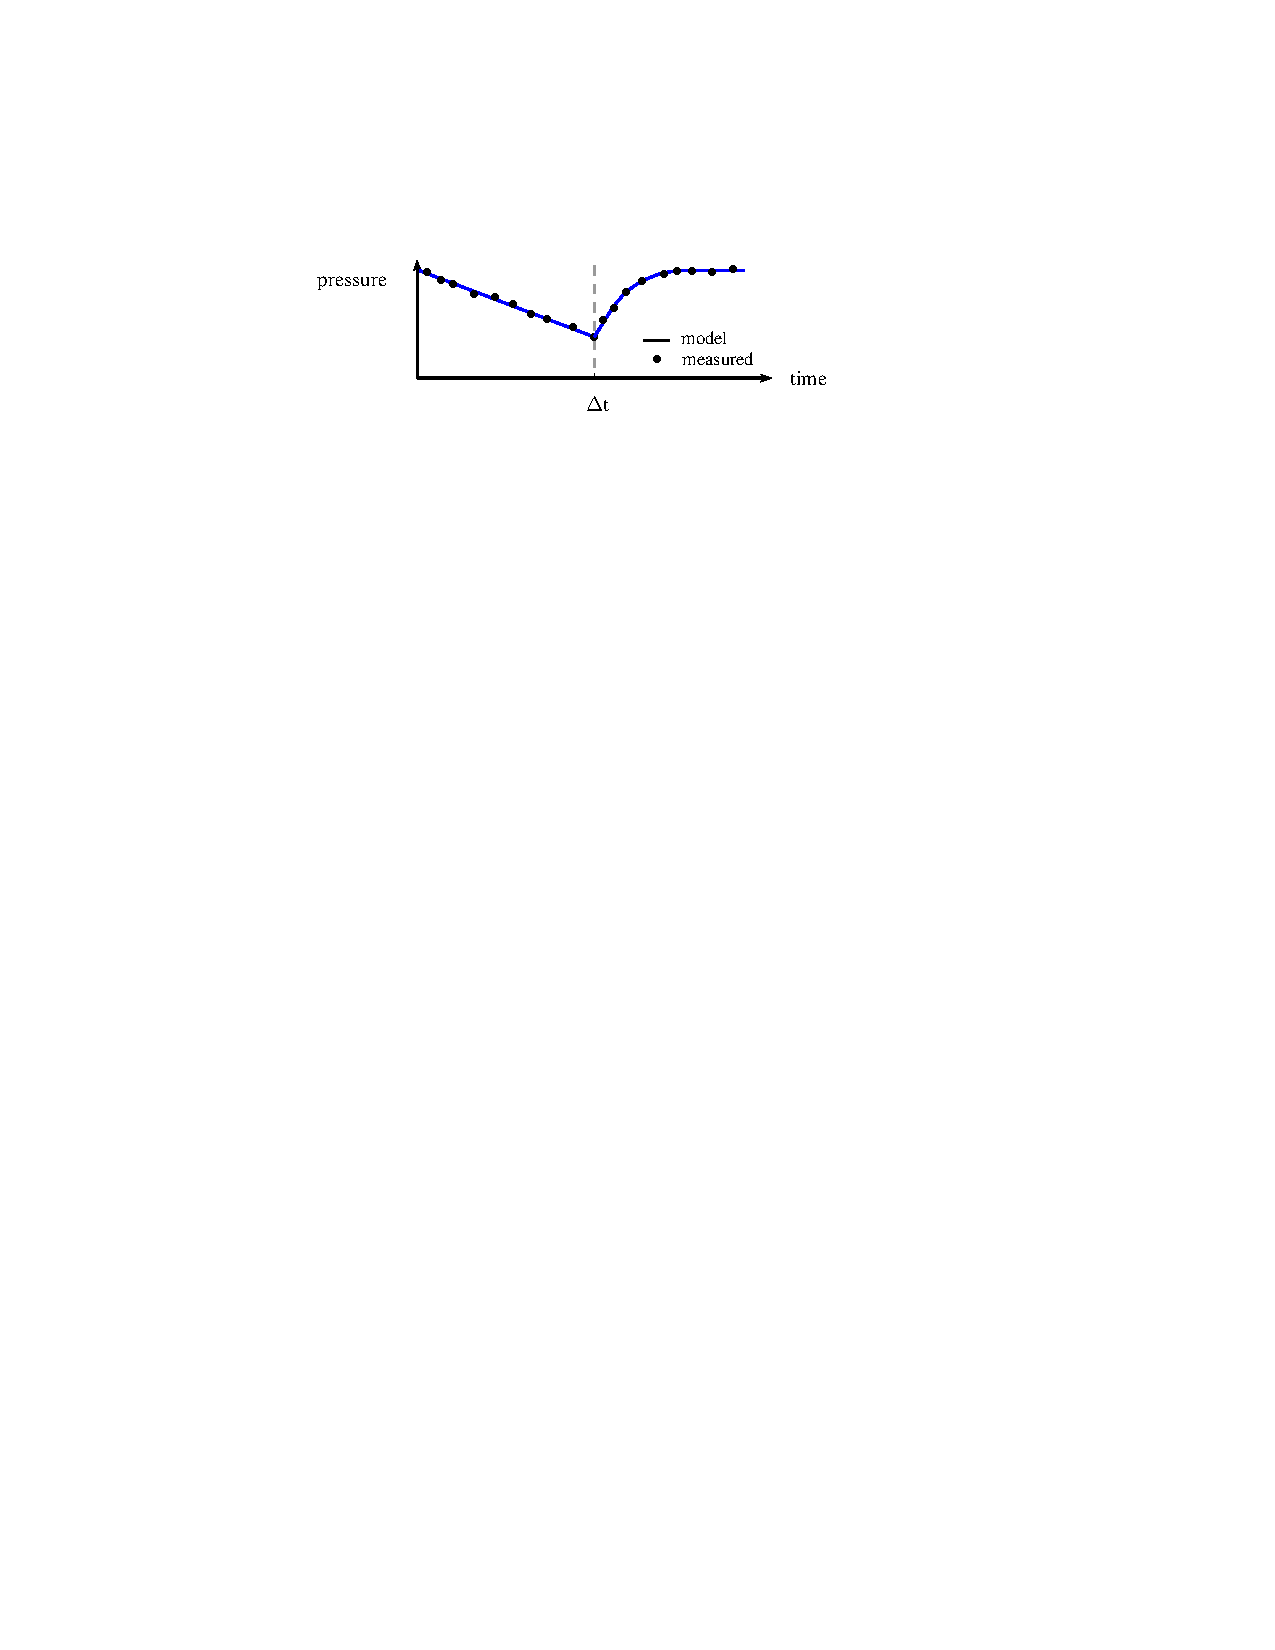
\includegraphics[scale=1]{Build_up.pdf}
        \end{center}
        \caption{Parameters estimated based on the analysis of buildup data.}
        \label{Build_up}
    \end{figure}

    \change[Murat \c{C}{\i}nar]{To illustrate an example of direct and inverse problems, let's consider single phase flow in a closed cylindrical reservoir produced by a single well at the center.}{Now we consider single phase flow in a cylindrical reservoir produced by a well at the center.} The\change[Murat \c{C}{\i}nar]{pd.E}{partial differential equation (p.d.e.)} describing the flow is given by,
    \begin{equation}
        \frac{1}{r}\frac{\partial }{\partial r}\left( \frac{kr}{\mu }\frac{\partial p}{\partial r} \right)=\phi {{c}_{t}}\frac{\partial p}{\partial t}
        \label{A}
    \end{equation}
    or if $k$, $\mu$ are constant,
    \begin{equation}
        \frac{1}{r}\frac{\partial }{\partial r}\left( r\frac{\partial p}{\partial r} \right)=\frac{\phi {{c}_{t}}\mu }{k}\frac{\partial p}{\partial t}=\frac{1}{\eta }\frac{\partial p}{\partial t}
        \label{B}
    \end{equation}

    \change[Murat \c{C}{\i}nar]{$\eta =\frac{\phi {{c}_{t}}\mu }{k}$}{$\eta =\frac{k}{\phi {{c}_{t}}\mu }$ } is the hydraulic diffusivity\change[Murat \c{C}{\i}nar]{which is}{;} a measure of the \change[Murat \c{C}{\i}nar]{rapidity with}{speed at} which a pressure disturbance \add[Murat \c{C}{\i}nar]{propagates} through the formation.
    If we specify, $k$, $\phi$, $c_{t}$, $\mu$, and the flow rate, then $p(r,t)$ is uniquely determined. This is an example for the \change[Murat \c{C}{\i}nar]{direct}{forward} problem.\\

    Inverse problem, given $q$ and $p$, \add[Murat \c{C}{\i}nar]{helps us to}
    \begin{enumerate}
        \item determine the p.d.e. that describes the reservoir best
        \item find $k$, $\phi$, etc.
    \end{enumerate}

    \remove[Murat \c{C}{\i}nar]{
    During the past ten years, a lot of work has been done to develop models to a wide variety of reservoir / well configurations such as fractures, layered reservoirs, multiple porosities (composite zones), fractured wells, slanted and horizontal wells, etc. Well testing literature is almost complete for single phase problems, but some work needs to be done for multi-phase problems and heterogeneous reservoir systems.\\

    Recently, people are much focused on the model recognition problem and the computer-aided parameter estimation by using non-linear regression techniques. Pressure derivatives and integrals are proven to be very useful in identifying the appropriate mathematical model from flow regime analysis. Currently, a lot of work is on artificial intelligence (AI) techniques for model recognition, such as rule-based expert and neural networks approaches.}

    \Trcknote[Murat \c{C}{\i}nar]{I added the following paragraph}Analytical solutions have been presented in the literature for a variety of different well and reservoir settings for single phase flow. A summary of these responses are given by Bourdet \cite{Bourdet_2002_1}.

    \begin{figure}
        \begin{center}
        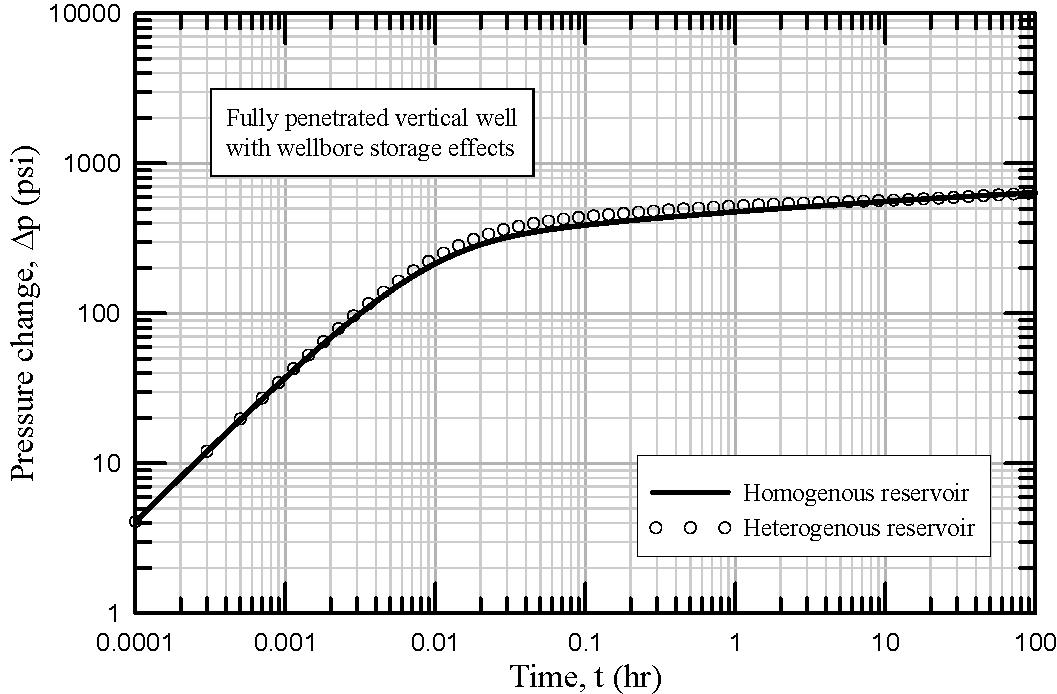
\includegraphics[scale=0.6]{Homogenous_vs_Heterogenous_dp.pdf}
        \end{center}
        \caption{Homogeneous vs heterogeneous reservoir, pressure difference .}
        \label{Homogenous_vs_Heterogenous_dp}
    \end{figure}

    \begin{figure}
        \begin{center}
        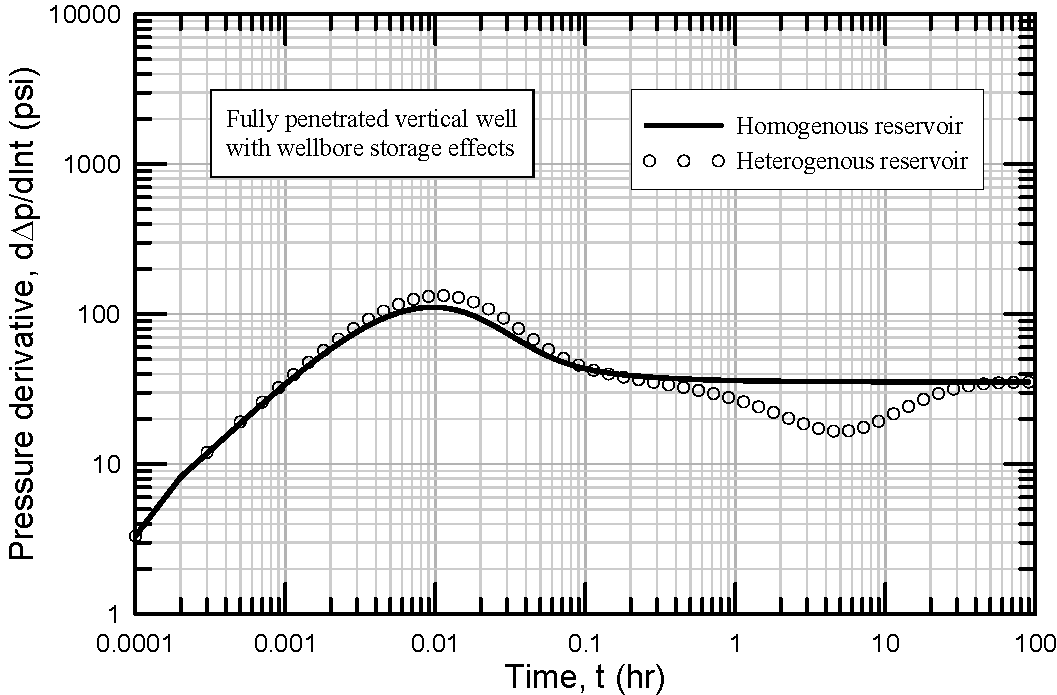
\includegraphics[scale=0.6]{Homogenous_vs_Heterogenous_dpder.pdf}
        \end{center}
        \caption{Homogeneous vs heterogeneous reservoir - logarithmic derivative.}
        \label{Homogenous_vs_Heterogenous_dpder}
    \end{figure}

    \begin{figure}
        \begin{center}
        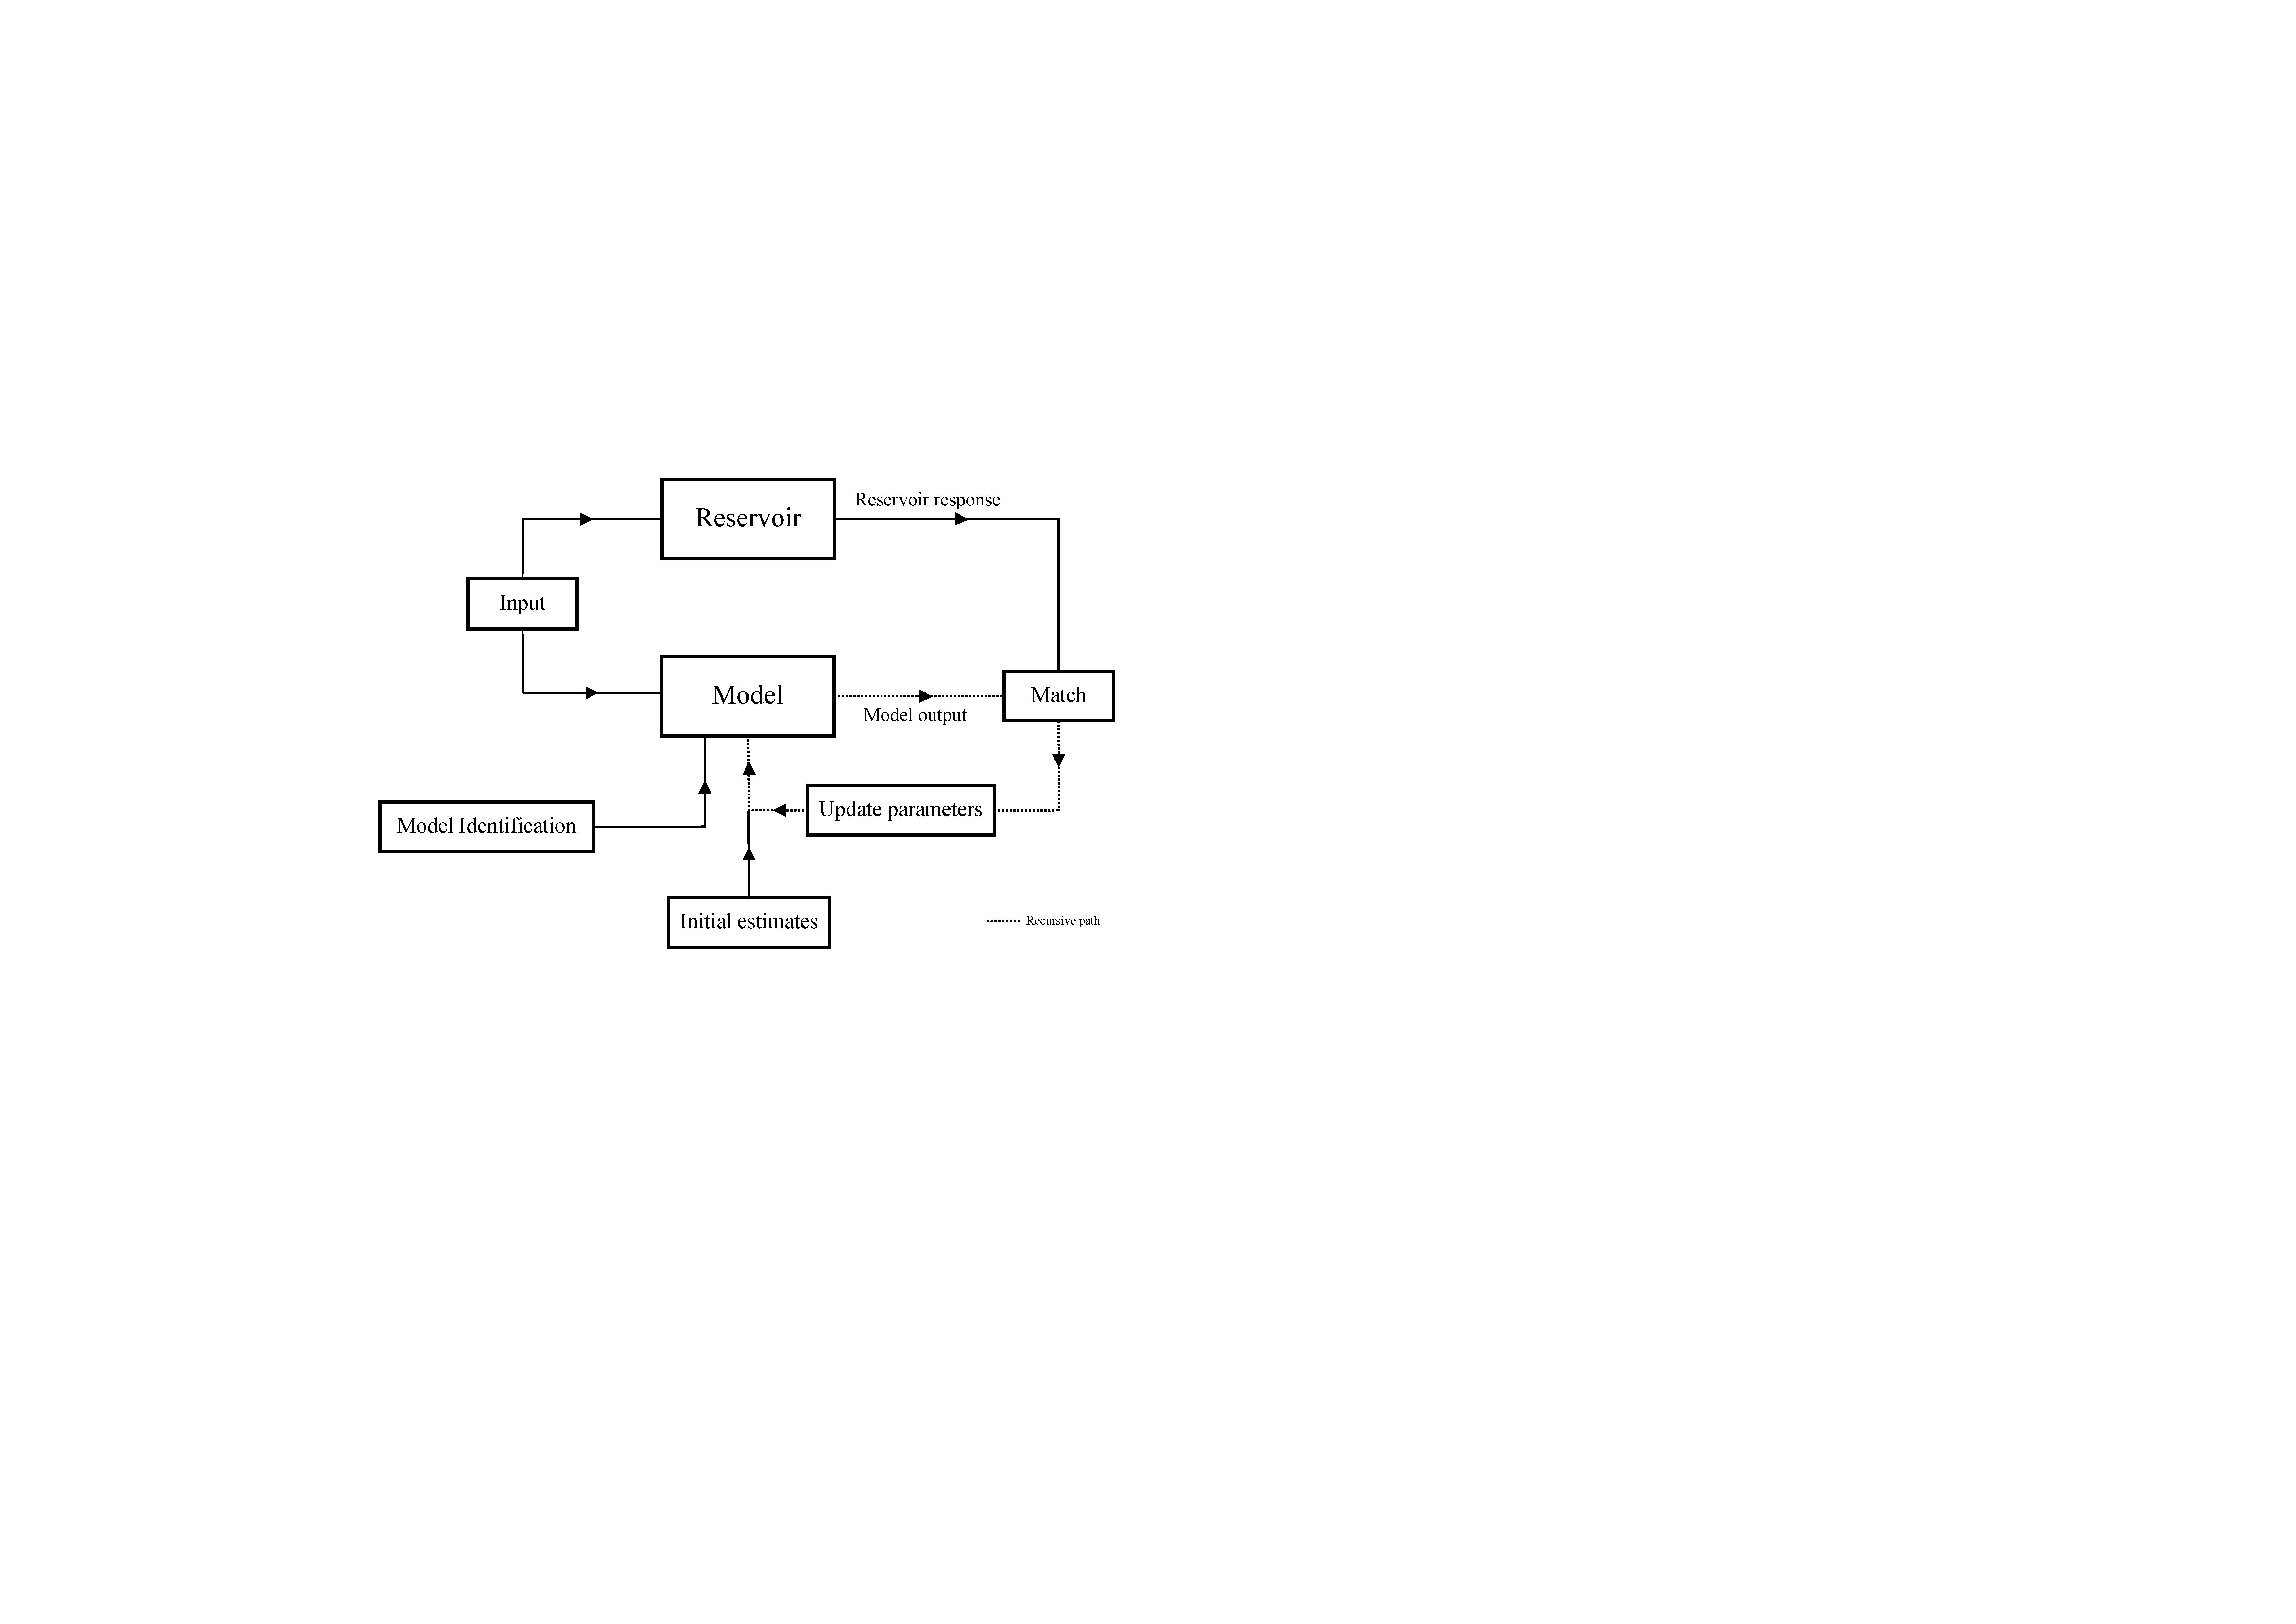
\includegraphics[scale=0.3]{Flow_Chart1.pdf}
        \end{center}
        \caption{Flow diagram of computer aided parameter estimation.}
        \label{Flow_Chart1}
    \end{figure}

    \section{Flow Equations}

    In this chapter, we will derive the equations which describe the fluid flow in porous media. Such equations are derived from the conservation of mass and the momentum equation as given by Darcy's semi-empirical equation. With the exception of thermal recovery schemes, all well-testing models assume isothermal conditions in the reservoir and thus the energy conservation is not needed.
    \subsection{Conservation of mass}
    For a single phase fluid \remove[Murat \c{C}{\i}nar]{(or a fluid composed of one hydrocarbon component)}, the mathematical form of the mass balance in porous media is given by
    \begin{equation}
        -\nabla \cdot \left( \rho \mathbf{v} \right)=\frac{\partial \left( \rho \phi  \right)}{\partial t}
        \label{continuity}
    \end{equation}
    \Trcknote[Murat \c{C}{\i}nar]{I removed the constant -5.615 from the equation}
    where $\rho$ is the density of the fluid in \change[Murat \c{C}{\i}nar]{$lbm/ft^{3}$}{$\mathbf{M}/\mathbf{L}^{3}$} and $\mathbf{v}$ is the fluid velocity vector in \change[Murat \c{C}{\i}nar]{$RB/ft^{2}day$}{$\mathbf{L}/\mathbf{T}$}. Note that the units of Eq. \ref{continuity} is \change[Murat \c{C}{\i}nar]{$lbm/ft^{3}day$}{$\mathbf{M}/\mathbf{L}^3\mathbf{T}$} It is also important to note that Eq. \ref{continuity} applies for any coordinate system and can be derived either from a mass balance done on a control volume for a coordinate system under consideration or from \remove[Murat \c{C}{\i}nar]{a} divergence theorem (or Gauss Theorem see Supplement II).

    In\change[Murat \c{C}{\i}nar]{x-y-x}{Cartesian} coordinate system,
    \begin{equation}
        \nabla \cdot \left( \rho \mathbf{v} \right)=\frac{\partial }{\partial x}\left( \rho {{v}_{x}} \right)+\frac{\partial }{\partial y}\left( \rho {{v}_{y}} \right)+\frac{\partial }{\partial z}\left( \rho {{v}_{z}} \right)
        \label{continuity_Cartesian}
    \end{equation}

    In\change[Murat \c{C}{\i}nar]{r-$\theta$-z}{cylindrical} coordinate system,
    \begin{equation}
        \nabla \cdot \left( \rho \mathbf{v} \right)=\frac{1}{r}\frac{\partial }{\partial r}\left( r\rho {{v}_{r}} \right)+\frac{1}{r}\frac{\partial }{\partial \theta }\left( \rho {{v}_{\theta }} \right)+\frac{\partial }{\partial z}\left( \rho {{v}_{z}} \right)
        \label{continuity_cylindrical}
    \end{equation}
    \Trcknote[Murat \c{C}{\i}nar]{typo in the equation corrected}
    \subsection{Conservation of momentum in porous media}
    The principle of momentum conservation is described by the equation of motion. For most hydrocarbon fluids, the shear stress - shear rate behavior \change[Murat \c{C}{\i}nar]{can be}{is} described by the Newton's law of friction, combined with the equation of motion, results in the well known Navier-Stokes equation. Solution of the Navier-Stokes equation with the appropriate boundary conditions yields the velocity distribution of a given problem. Although, it is possible to solve Navier-Stokes in pipe flow, it is almost impossible to solve due to complexity of the pore geometry and its distribution. This hinders the formation of the boundary conditions for flow through a porous medium. Therefore, a different approach \change[Murat \c{C}{\i}nar]{must be}{is} taken. In 1856, \change[Murat \c{C}{\i}nar]{a French hydraulic engineer Henry} Darcy discovered that \change[Murat \c{C}{\i}nar]{the velocity vector and the pressure gradient for a single phase viscous flow}{for a single phase viscous flow in porous media, the velocity is proportional to the pressure gradient with a proportionality constant $k$. The general form of Darcy's Law including gravity effects is given by Eq.}\ref{Darcy's_Law}.
    \begin{equation}
        \mathbf{v}=-\frac{\mathbf{k}}{\mu }\left( \nabla p-\rho g\nabla z' \right)
        \label{Darcy's_Law}
    \end{equation}
    \Trcknote[Murat \c{C}{\i}nar]{I removed the filed unit constants}
    where $\mathbf{v}$ is defined as a volumetric flow rate across a unit cross-section area (solid+fluid) averaged over a small region of space. The unit of $\mathbf{v}$ is in \change[Murat \c{C}{\i}nar]{$RB/ft^{2}day$}{$\mathbf{L}/\mathbf{T}$}. Eq. \ref{Darcy's_Law} yield\add[Murat \c{C}{\i}nar]{s} a velocity vector \change[Murat \c{C}{\i}nar]{which}{that} replaces the solution of Navier-Stokes equation. In Eq. \ref{Darcy's_Law} $\mathbf{k}$ is \change[Murat \c{C}{\i}nar]{a}{the} permeability tensor. Operationally, $\mathbf{k}$ acts like a matrix in \change[Murat \c{C}{\i}nar]{x-y-z}{coordinate system}, we usually \change[Murat \c{C}{\i}nar]{use}{assume}
    \begin{equation*}
        \mathbf{k}\,\nabla p=\begin{bmatrix}
             {{k}_{x}} & 0 & 0  \\
             0 & {{k}_{y}} & 0  \\
             0 & 0 & {{k}_{z}}  \\
            \end{bmatrix}\begin{bmatrix}
            & \frac{\partial p}{\partial x} \\
            & \frac{\partial p}{\partial y} \\
            & \frac{\partial p}{\partial z} \\
            \end{bmatrix} = \begin{bmatrix}
            & {{k}_{x}}\frac{\partial p}{\partial x} \\
            & {{k}_{y}}\frac{\partial p}{\partial y} \\
            & {{k}_{z}}\frac{\partial p}{\partial z} \\
            \end{bmatrix}
        \label{Permeability_Tensor}
    \end{equation*}
    \begin{equation*}
        \nabla {z}'=\begin{bmatrix}
        & \frac{\partial {z}'}{\partial x} & \\
        & \frac{\partial {z}'}{\partial y} & \\
        &\frac{\partial {z}'}{\partial z}  &
        \end{bmatrix}
        \label{Z}
    \end{equation*}
    where, ${z}'$ is the direction in which gravity acts, i.e., the direction towards the center of the earth.
    In \change[Murat \c{C}{\i}nar]{x-y-z}{Cartesian} coordinate system, \remove[Murat \c{C}{\i}nar]{Eq. 2.5} for each velocity component,
    \begin{equation}
    {{v}_{\xi }}=-\frac{{{k}_{\xi }}}{\mu }\left( \frac{\partial p}{\partial \xi }-\rho g\frac{\partial z'}{\partial \xi } \right),\quad \xi =x,y,z
        \label{Darcy_velocity}
    \end{equation}

    We generally denote $\gamma$ as the specific weight of fluid and define as,
    \begin{equation*}
        \gamma =\rho g
        \label{Specific_weight}
    \end{equation*}

    It follows from Eq. \ref{Darcy_velocity}, \ref{continuity_Cartesian}, and \ref{continuity} that the p.d.e. describing conservation of mass in \remove[Murat \c{C}{\i}nar]{x-y-z}{Cartesian} coordinate system is
    \begin{equation}
        \begin{split}
            & \,\,\,\,\,\,\ \frac{\partial }{\partial x}\left[ \rho \frac{{{k}_{x}}}{\mu }\left( \frac{\partial p}{\partial x}-\gamma \frac{\partial z'}{\partial x} \right) \right] \\
            & +\frac{\partial }{\partial y}\left[ \rho \frac{{{k}_{y}}}{\mu }\left( \frac{\partial p}{\partial y}-\gamma \frac{\partial z'}{\partial y} \right) \right] \\
            & +\frac{\partial }{\partial z}\left[ \rho \frac{{{k}_{z}}}{\mu }\left( \frac{\partial p}{\partial z}-\gamma \frac{\partial z'}{\partial z} \right) \right]=\frac{\partial }{\partial t}\left( \rho \phi  \right) \\
        \end{split}
    \label{Continuity_Darcy}
    \end{equation}

    In \change[Murat \c{C}{\i}nar]{r-z}{Cylindrical} coordinates (neglecting flow in $\theta$ direction)
    \begin{equation}
        \,\,\,\,\,\frac{1}{r}\,\frac{\partial }{\partial r}\left[ r\frac{{{k}_{r}}}{\mu }\rho \left( \frac{\partial p}{\partial r}-\gamma \frac{\partial z'}{\partial r} \right) \right]+\frac{\partial }{\partial z}\left[ \frac{{{k}_{z}}}{\mu }\rho \left( \frac{\partial p}{\partial z}-\gamma \frac{\partial z'}{\partial z} \right) \right]=\frac{\partial }{\partial t}\left( \rho \phi  \right)
    \label{Continuity_Darcy_Cylindrical}
    \end{equation}

    \vspace{15pt}
    \large{\textbf{Remark on gravity term:}}\\
    \rule{\textwidth}{1pt}
    \begin{figure}
        \begin{center}
            \includegraphics[scale=1]{Z_Aside.pdf}
        \end{center}
        \label{Z_Aside}
    \end{figure}
    In \change[Murat \c{C}{\i}nar]{r-$\theta$-z}{Cylindrical} coordinates,\change[Murat \c{C}{\i}nar]{if reservoir is horizontal; i.e. $\theta'=0$}{assume $z$ and $z'$ are in the same direction then,}
    \begin{equation*}
        \frac{\partial z'}{\partial r}=\frac{\partial z'}{\partial \theta }=0\quad and\quad \frac{\partial z'}{\partial z}=1
    \end{equation*}
    \change[Murat \c{C}{\i}nar]{If we had a dip angle $\theta'$}{if the reservoir is dipping with an angle of $\theta'$},
    \begin{equation*}
        \frac{\partial z'}{\partial r}=\sin \theta '\quad \frac{\partial z'}{\partial \theta }=\cos \theta '\quad \frac{\partial z'}{\partial z}=\cos \theta '
    \end{equation*}\\
    \rule{\textwidth}{1pt}\\
    \vspace{15pt}

    \change[Murat \c{C}{\i}nar]{If we}{Now} consider a single well \change[Murat \c{C}{\i}nar]{in}{at} the center of a cylindrical reservoir, then Eq. \ref{Continuity_Darcy_Cylindrical} correctly describes the fluid flow for both partially penetrating and fully penetrating cases, see Fig \ref{PartialvsFullPenet}.\\
    \begin{figure}
        \begin{center}
        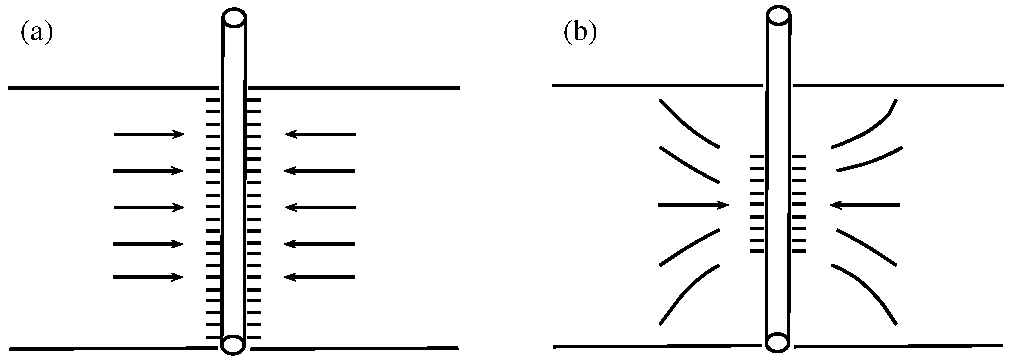
\includegraphics[scale=0.6]{PartialvsFullPenet.pdf}
        \end{center}
        \caption{(a) Fully penetrated vertical well. (b) Partially penetrated vertical well.}
        \label{PartialvsFullPenet}
    \end{figure}
    \remove[Murat \c{C}{\i}nar]{Recalling our general continuity equation for the single phase flow gives,}
    \add[Murat \c{C}{\i}nar]{Now define formation volume factor $B$ as,}

    \begin{equation}
        B=\frac{{{V}_{reservoir}}}{{{V}_{SC}}}=\frac{{m}/{\rho }\;}{{{{m}/{\rho }\;}_{SC}}}=\frac{{{\rho }_{SC}}}{\rho }\quad ;\quad {{\rho }_{SC}}\,\text{is}\,\text{constant}
    \label{Formation_Volume_Factor}
    \end{equation}

    \remove[Murat \c{C}{\i}nar]{which we call it as Formation volume factor, then we can write Equation (2.8) as}
    \add[Murat \c{C}{\i}nar]{Recall general continuity equation,} Eq. \ref{continuity} and insert Eq. \ref{Formation_Volume_Factor}, then we have,

    \begin{equation}
        -\nabla \cdot \left( \frac{\mathbf{v}}{B} \right)=\frac{\partial }{\partial t}\left( \frac{\phi }{B} \right)
    \label{Continuity_B}
    \end{equation}

    $B=B(p)$, $\rho=\rho(p)$, and $\phi=\phi(p)\rightarrow$ single valued functions of $p$
    \add[Murat \c{C}{\i}nar]{Expanding right hand side (RHS) of} Eq. \ref{Continuity_B},

    \begin{equation}
        \begin{split}
            \frac{\partial }{\partial t}\left( \frac{\phi }{B} \right)&= \phi \frac{\partial }{\partial t}\left( \frac{1}{B} \right)+\frac{1}{B}\frac{\partial \phi }{\partial t} \\
            &=\phi \left( -\frac{1}{{{B}^{2}}}\frac{dB}{dp} \right)\frac{\partial p}{\partial t}+\frac{1}{B}\frac{d\phi }{dt}\frac{\partial p}{\partial t} \\
            &=\frac{\phi }{B}\left( -\frac{1}{B}\frac{dB}{dp}+\frac{1}{\phi}\frac{d\phi }{dt} \right)\frac{\partial p}{\partial t} \\
    \end{split}
    \label{Continuity_B_Expand_RHS}
    \end{equation}
    \Trcknote[Murat \c{C}{\i}nar]{Typo in Eq corrected.}
    \remove[Murat \c{C}{\i}nar]{but} Fluid and rock compressibilities are defined, respectively, by,

    \begin{equation}
    {{c}_{fluid}}=-\frac{1}{V}\frac{dV}{dp}=-\frac{1}{B}\frac{dB}{d\rho }=\frac{1}{\rho }\frac{d\rho }{dp}
    \label{Fluid_compressibility}
    \end{equation}

    \begin{equation}
    {{c}_{r}}={{c}_{f}}=\frac{1}{\phi }\frac{d\phi }{dp}
    \label{Rock_compressibility}
    \end{equation}

    (here $p$ is the fluid pressure in the pore, therefore, $\frac{d\phi }{dp}>0$.) \\
    Using Eqs. \ref{Fluid_compressibility} and \ref{Rock_compressibility} in Eq. \ref{Continuity_B_Expand_RHS} and the resulting equation in Eq. \ref{Continuity_B} gives,

    \begin{equation}
        -\nabla \cdot \left( \frac{\mathbf{v}}{B} \right)=\frac{\phi {{c}_{t}}}{B}\frac{\partial p}{\partial t}
    \label{Continuity_B_ct}
    \end{equation}

    \add[Murat \c{C}{\i}nar]{Note that here the total compressibility $c_{t}$ is defined as ${{ c }_{t}}={{c}_{fluid}}+{{c}_{r}}$. Under the assumptions of Darcy's Law we have,}

    \begin{equation}
        \nabla \cdot \left( \frac{\mathbf{k}}{\mu B}\left( \nabla p-\gamma\nabla z' \right) \right)=\frac{\phi {{c}_{t}}}{B}\frac{\partial p}{\partial t}
    \label{Continuity_B_ct_Darcy}
    \end{equation}

    \subsubsection{Slightly compressible fluid of constant compressibility}

    Now assuming negligible gravity effects and $k/\mu$ is constant then,

    \begin{equation}
        \frac{k}{\mu }\nabla \cdot \left( \rho \nabla p \right)=\phi {{c}_{t}}\rho \frac{\partial p}{\partial t}
    \label{Continuity_B_ct_Darcy_No_Gravity1}
    \end{equation}

    \change[Murat \c{C}{\i}nar]{If we assume}{Assuming} $c{{\left( \nabla p \right)}^{2}}$ is small here $c=\frac{1}{\rho }\frac{\partial \rho }{\partial p}$, Eq. \ref{Continuity_B_ct_Darcy_No_Gravity1} is well approximated by

    \begin{equation}
        \frac{k}{\mu }{{\nabla }^{2}}p=\phi {{c}_{t}}\frac{\partial p}{\partial t}
    \label{Continuity_B_ct_Darcy_No_Gravity1_approx}
    \end{equation}

    \vspace{15pt}
    \large{\textbf{Remark on coordinate systems:}}\\
    \rule{\textwidth}{1pt}

    \begin{equation*}
        {{\nabla }^{2}}p=\frac{{{\partial }^{2}}p}{\partial {{x}^{2}}}+\frac{{{\partial }^{2}}p}{\partial {{y}^{2}}}+\frac{{{\partial }^{2}}p}{\partial {{z}^{2}}}\quad \text{in Cartesian coordinates}
    \label{Laplacian_Cartesian}
    \end{equation*}

    \begin{equation*}
        {{\nabla }^{2}}p=\frac{1}{r}\frac{\partial }{\partial r}\left( r\frac{\partial p}{\partial r} \right)+\frac{1}{{{r}^{2}}}\frac{{{\partial }^{2}}p}{\partial {{\theta }^{2}}}+\frac{{{\partial }^{2}}p}{\partial {{z}^{2}}}\quad \text{in cylindrical coordinates}
    \label{Laplacian_Cylindrical}
    \end{equation*}

    \begin{equation*}
        \begin{split}
    & {{\nabla }^{2}}p=\frac{1}{{{r}^{2}}}\frac{\partial }{\partial r}\left( {{r}^{2}}\frac{\partial p}{\partial r} \right)+\frac{1}{{{r}^{2}}sin\theta }\frac{\partial }{\partial \theta }\left( sin\theta \frac{\partial p}{\partial \theta } \right) \\
    & +\frac{1}{{{r}^{2}}si{{n}^{2}}\theta }\frac{{{\partial }^{2}}p}{\partial {{\phi }^{2}}} \\
    \end{split}\quad \text{in spherical coordinates}
    \label{Laplacian_Spherical}
    \end{equation*}

    \begin{figure}[H]
        \begin{center}
            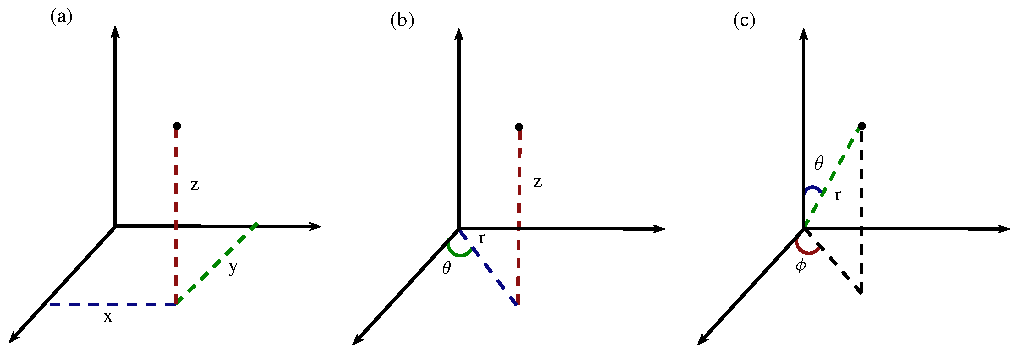
\includegraphics[scale=0.65]{Coordinates.pdf}
        \end{center}
        \caption{(a) Cartesian coordinates. (b) Cylindrical coordinates. (c) Spherical coordinates.}
        \label{Coordinates}
    \end{figure}
    \rule{\textwidth}{1pt}
    \vspace{15pt}

    Further \change[Murat \c{C}{\i}nar]{if we assume}{assuming},
    \begin{equation}
        c=\frac{1}{\rho }\frac{\partial \rho }{\partial p}=\text{constant}
    \label{c_constant}
    \end{equation}

    \begin{equation*}
        \int_{{{p}_{i}}}^{p}{cdp}=\int_{{{\rho }_{i}}}^{\rho }{\frac{1}{\rho }d\rho }
    \end{equation*}

    \begin{equation*}
        c\left( p-{{p}_{i}} \right)=\ln \left( \frac{\rho }{{{\rho }_{i}}} \right)\quad ; \quad p_{i}\,\text{initial pressure}
    \end{equation*}
    or
    \begin{equation}
        \rho ={{\rho }_{i}}\exp \left[ -c\left( {{p}_{i}}-p \right) \right]
    \label{rho_func}
    \end{equation}

    Using Taylor series representation of $\exp \left[ -c\left( {{p}_{i}}-p \right) \right]$ gives,
    \begin{equation*}
        \begin{split}
         \rho &={{\rho }_{i}}\left[ 1-c\left( {{p}_{i}}-p \right)+\frac{{{c}^{2}}}{2}{{\left( {{p}_{i}}-p \right)}^{2}}+\cdots  \right] \\
        & ={{\rho }_{i}}\left[ 1-c\left( {{p}_{i}}-p \right)+\frac{{{c}^{2}}}{2}{{\left( {{p}_{i}}-\widetilde{p} \right)}^{2}} \right]\quad p<\widetilde{p}<{{p}_{i}} \\
        \end{split}
    \end{equation*}
    \begin{equation}
        \rho ={{\rho }_{i}}\left[ 1-c\left( {{p}_{i}}-p \right) \right]
    \label{rho_func_2}
    \end{equation}
    \add[Murat \c{C}{\i}nar]{Note that} $c$ is very small for oil (or liquids); $c\approx10^{-5}\sim10^{-6}$. Using Eq. \ref{rho_func_2} in Eq. \ref{Continuity_B_ct_Darcy_No_Gravity1_approx}.
    \begin{equation}
        \frac{k}{\mu }{{\nabla }^{2}}p = \phi {{c}_{t}}\frac{\partial p}{\partial t}
    \label{Continuity_B_ct_Darcy_No_Gravity1_approx_rho}
    \end{equation}

    \subsection{Multiphase flow}
    Three distinct phases, gas, oil, and water occur i a petroleum reservoir. Varying pressure conditions (isothermal system assumed) cause a mass exchange between \remove[Murat \c{C}{\i}nar]{the}two hydrocarbon phases \add[Murat \c{C}{\i}nar]{- oil-gas} (water-oil and gas-water systems \change[Murat \c{C}{\i}nar]{can be}{is} assumed immiscible). The \change[Murat \c{C}{\i}nar]{material}{mass} transfer between oil and gas is described by solution gas-oil ration, $R_{s}$, which gives the amount of gas dissolved in oil as a function of pressure, i.e. $[V_{dissolved \, gas}/V_{o}]_{STC}$.\\

    The fluid flow equations (based on $\beta$-model) with the introduction of phase saturations for oil-water-gas system \change[Murat \c{C}{\i}nar]{can be}{is} written as;

    \begin{equation}
    -\nabla \cdot \left( \frac{\mathbf{v}_{o}}{{{B}_{o}}} \right)=\frac{\partial }{\partial t}\left( \frac{\phi {{S}_{o}}}{{{B}_{o}}} \right)\quad for\,oil
    \label{Continuity_oil}
    \end{equation}

    \begin{equation}
    -\nabla \cdot \left( \frac{\mathbf{v}_{w}}{{{B}_{w}}} \right)=\frac{\partial }{\partial t}\left( \frac{\phi {{S}_{w}}}{{{B}_{w}}} \right)\quad for\,water
    \label{Continuity_water}
    \end{equation}

    \begin{equation}
    -\nabla \cdot \left( \frac{{{R}_{s}}{{\mathbf{v}}_{o}}}{{{B}_{o}}}+\frac{{{\mathbf{v}}_{g}}}{{{B}_{g}}} \right)=\frac{\partial }{\partial t}\left[ \phi \left( \frac{{{R}_{s}}}{{{B}_{o}}}{{S}_{o}}+\frac{{{S}_{g}}}{{{B}_{g}}} \right) \right]\quad for\,gas
    \label{Continuity_gas}
    \end{equation}

    With introducing relative permeability \remove[Murat \c{C}{\i}nar]{concept}, the velocity vector for each phase is given by,

    \begin{equation}
    {{\mathbf{v}}_{\varphi}}=-\frac{\mathbf{k}\,{{k}_{r\varphi}}}{{{\mu }_{\varphi}}}\left( \nabla {{p}_{\varphi}}-{{\gamma }_{\varphi}}\nabla z' \right)
    \label{Darcy_multiphase}
    \end{equation}

    where $\varphi = o, w, or g$.\\

    Using Eq. \ref{Darcy_multiphase} in Eqs. \ref{Continuity_oil}, \ref{Continuity_water}, and \ref{Continuity_gas} for corresponding \change[Murat \c{C}{\i}nar]{Hydro Carbon component}{phase},

    \begin{equation}
    \nabla \cdot \left( \frac{\mathbf{k}\,{{k}_{ro}}}{{{B}_{o}}{{\mu }_{o}}}\left( \nabla {{p}_{o}}-{{\gamma }_{o}}\nabla z' \right) \right)=\frac{\partial }{\partial t}\left( \frac{\phi {{S}_{o}}}{{{B}_{o}}} \right)
    \label{Continuity_oil_Darcy}
    \end{equation}

    \begin{equation}
    \nabla \cdot \left( \frac{\mathbf{k}\,{{k}_{rw}}}{{{B}_{w}}{{\mu }_{w}}}\left( \nabla {{p}_{w}}-{{\gamma }_{w}}\nabla z' \right) \right)=\frac{\partial }{\partial t}\left( \frac{\phi {{S}_{w}}}{{{B}_{w}}} \right)
    \label{Continuity_water_Darcy}
    \end{equation}

    \begin{equation}
    \begin{split}
    & \nabla \cdot \left( \frac{{{R}_{s}}\mathbf{k}\,{{k}_{ro}}}{{{B}_{o}}{{\mu }_{o}}}\left( \nabla {{p}_{o}}-{{\gamma }_{o}}\nabla z' \right)+\frac{\mathbf{k}\,{{k}_{rg}}}{{{B}_{g}}{{\mu }_{g}}}\left( \nabla {{p}_{g}}-{{\gamma }_{g}}\nabla z' \right) \right) \\
    & \quad \quad \quad \quad \quad \quad \quad \quad \quad \quad \quad =\frac{\partial }{\partial t}\left[ \phi \left( \frac{{{R}_{s}}}{{{B}_{o}}}{{S}_{o}}+\frac{{{S}_{g}}}{{{B}_{g}}} \right) \right] \\
    \end{split}
    \label{Continuity_gas_Darcy}
    \end{equation}

    \begin{figure}
        \begin{center}
        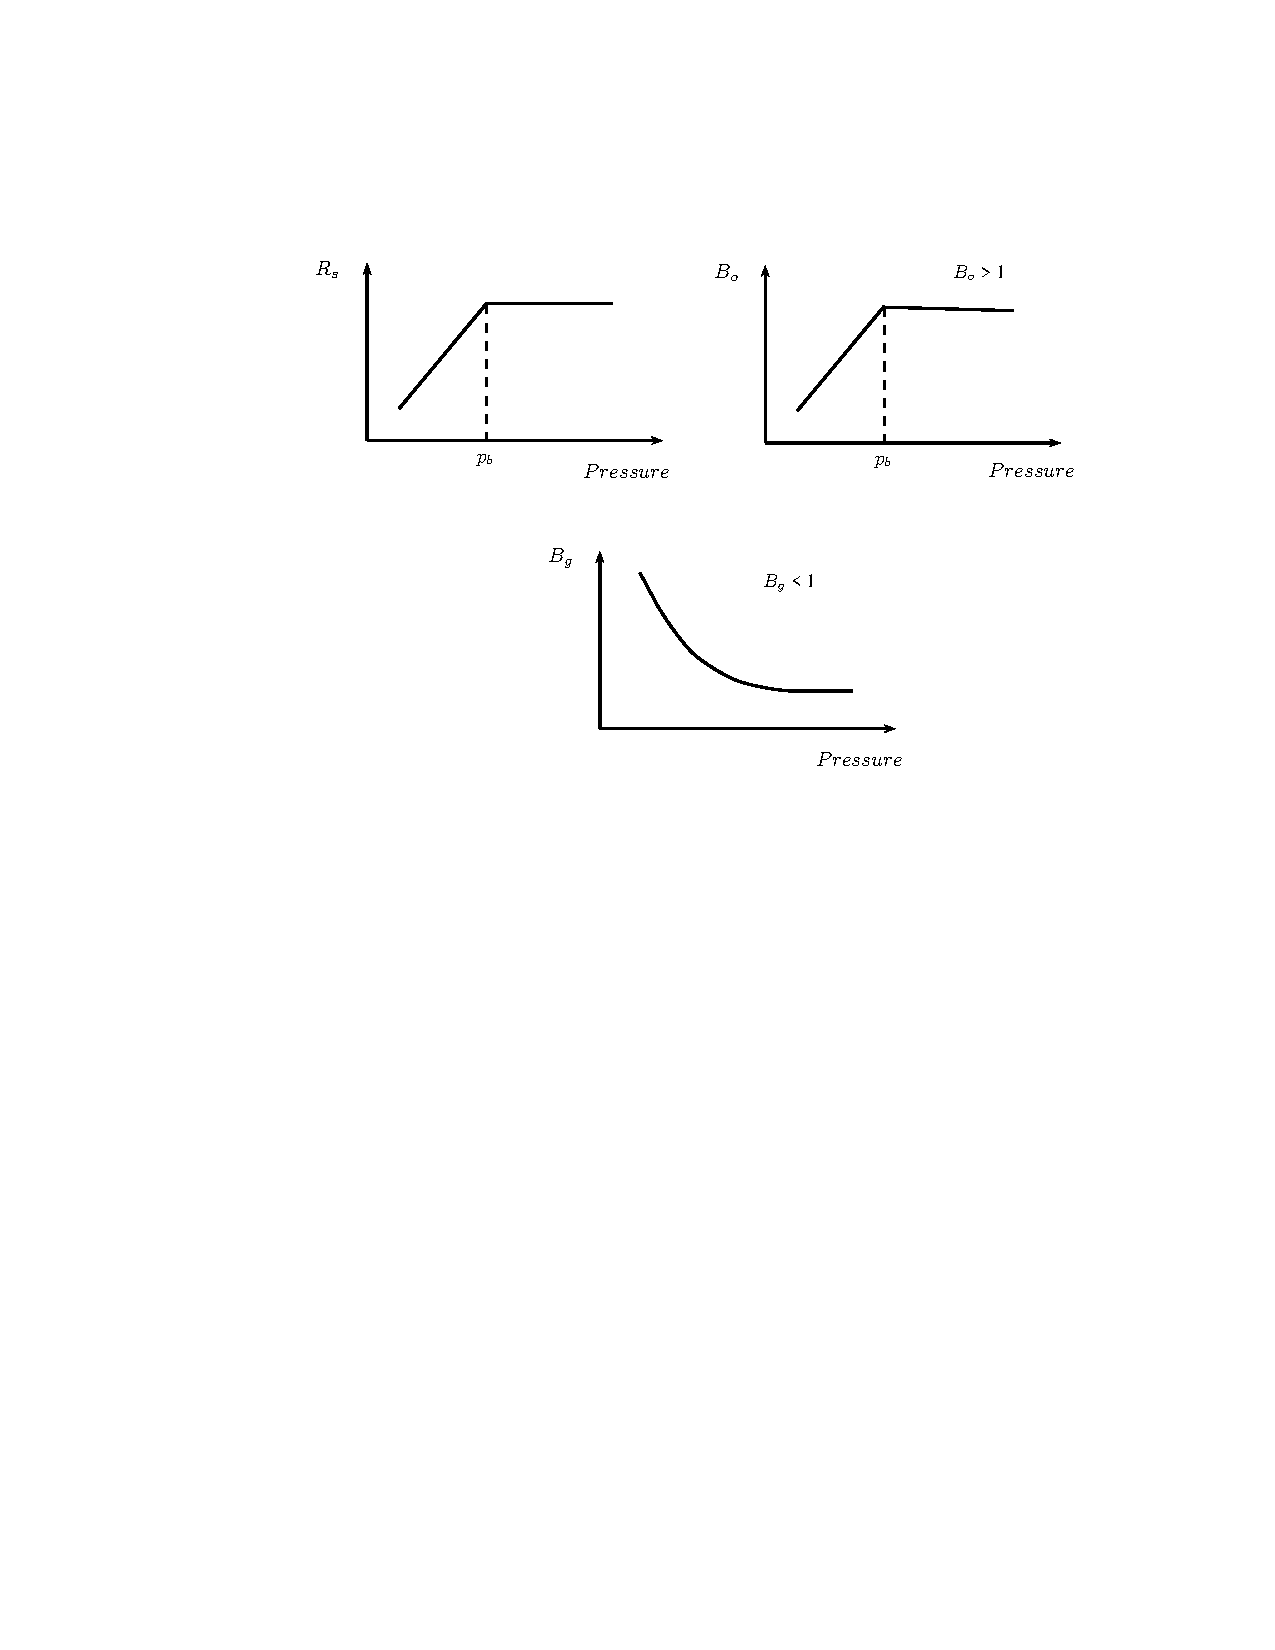
\includegraphics[scale=0.9]{Rs_Bo_Bg.pdf}
        \end{center}
        \caption{$R_{s}$, $B_{o}$, $B_{g}$ behavior.}
        \label{Rs_Bo_Bg}
    \end{figure}

    It is important to note that $B$ defined by Eq. \ref{Formation_Volume_Factor}\add[Murat \c{C}{\i}nar]{,} considering oil, \remove[Murat \c{C}{\i}nar]{this} is \change[Murat \c{C}{\i}nar]{correct}{valid} if \change[Murat \c{C}{\i}nar]{we have a}{oil is} single component or \remove[Murat \c{C}{\i}nar]{if we are talking about} "black-oil" with no dissolved gas ($R_{s}=0$). \change[Murat \c{C}{\i}nar]{However}{On the other hand}, Eq. \ref{Continuity_B_ct_Darcy} is \change[Murat \c{C}{\i}nar]{correct}{valid} for black-oil problems with $R_{s}\neq0$ provided that \change[Murat \c{C}{\i}nar]{we are}{the pressure is} above bubble-point. \remove[Murat \c{C}{\i}nar]{If we are above bubble-point,}Eq. \ref{Continuity_oil_Darcy} and Eq. \ref{Continuity_gas_Darcy} \change[Murat \c{C}{\i}nar]{will be}{becomes} identical\add[Murat \c{C}{\i}nar]{ if the pressure is above bubble point}.

    \change[Murat \c{C}{\i}nar]{Sometimes we write the flow equation}{In some cases, the flow equation is written} in terms of pseudo potential.

    \begin{equation}
        \psi =\int_{{{p}_{0}}}^{p}{\frac{1}{\gamma }dp}-\left( z'-{{z}_{0}}' \right)
    \label{Pseudo_Potential}
    \end{equation}

    where $z'$ is measured positive in the direction of gravity and ${{z}_{0}}'$ is the datum where \remove[Murat \c{C}{\i}nar]{we take as reference}${{p}_{0}}$ \add[Murat \c{C}{\i}nar]{is measured}. Also $\gamma=\mathbf{M}/\mathbf{L}^{2}\mathbf{T}^{2})$ and $\gamma=\gamma(p)$.

    \begin{equation*}
        \begin{split}
             \nabla \psi & =\nabla \int_{{{p}_{0}}}^{p}{\frac{1}{\gamma }dp}-\nabla \left( z'-{{z}_{0}}' \right) \\
            & =\frac{d}{dp}\left\{ \int_{{{p}_{0}}}^{p}{\frac{1}{\gamma }dp} \right\}\nabla p-\nabla z' \\
            & =\frac{1}{\gamma }\nabla p-\nabla z' \\
        \end{split}
    \end{equation*}

    Then,

    \begin{equation}
        \gamma \,\nabla \psi =\nabla p-\gamma \,\nabla z'
    \label{Pseudo_Potential_1}
    \end{equation}

    and

    \begin{equation}
        \frac{\partial \psi }{\partial t}=\frac{1}{\gamma }\frac{\partial p}{\partial t}
    \label{Pseudo_Potential_2}
    \end{equation}

    Using Eqs. \ref{Pseudo_Potential_1} and \ref{Pseudo_Potential_2} in Eq. \ref{Continuity_B_ct_Darcy} we obtain,

    \begin{equation}
        \nabla \cdot \left( \frac{\mathbf{k}\gamma }{B\mu }\nabla \psi  \right)=\frac{\phi {{c}_{t}}\gamma }{B}\frac{\partial \psi }{\partial t}
    \label{Pseudo_Potential_Final}
    \end{equation}

    If we consider that we have stress dependent reservoir, that is permeability decreases as the fluid pressure in the pores decreases, then
    \begin{equation*}
        \mathbf{k}=k\left( p \right)\widetilde{\mathbf{k}}
    \end{equation*}
        where the entries of $\widetilde{\mathbf{k}}$ are independent of pressure. It has been observed that tight (and geothermal) reservoirs are \remove[Murat \c{C}{\i}nar]{good} examples of stress dependent reservoirs. Then Eq. \ref{Pseudo_Potential_Final} \change[Murat \c{C}{\i}nar]{can be}{is} expressed as

    \begin{equation}
        \nabla \cdot \left( \frac{k\left( p \right)\widetilde{\mathbf{k}}\gamma }{B\mu }\nabla \psi  \right)=\frac{\phi {{c}_{t}}\gamma }{B}\frac{\partial \psi }{\partial t}
    \label{Pseudo_Potential_Final_Stress_dependent}
    \end{equation}
    \remove[Murat \c{C}{\i}nar]{
    It is important to note that Eq. 2.38 is non-linear because $\phi$, $c_{t}$, $\gamma$, $\mu$, $B$, and $k$ are all pressure dependent (or potential). To partially linearize the Eq. 2.38 (or Eq. 2.14), we normally define a pseudo pressure function if gravity effects are not important.}
    \Trcknote[Murat \c{C}{\i}nar]{Following paragraph is added.}A pseudo pressure function is defined to partially linearize Eq. \ref{Pseudo_Potential_Final_Stress_dependent} (or Eq. \ref{Continuity_B_ct_Darcy}) under the assumption that the gravity effects are not important.

    \begin{equation}
        m\left( p \right)=\int_{{{p}_{0}}}^{p}{\frac{k\left( p \right)}{\mu \left( p \right)B\left( p \right)}dp}
    \label{Pseudo_Pressure}
    \end{equation}

    \begin{equation}
        \nabla m\left( p \right)=\frac{d}{dp}m\left( p \right)\nabla p=\frac{k\left( p \right)}{\mu \left( p \right)B\left( p \right)}\nabla p
    \label{Pseudo_Pressure_1}
    \end{equation}

    \begin{equation}
        \frac{\partial m\left( p \right)}{\partial t}=\frac{k\left( p \right)}{\mu \left( p \right)B\left( p \right)}\frac{\partial p}{\partial t}
    \label{Pseudo_Pressure_2}
    \end{equation}

    If \change[Murat \c{C}{\i}nar]{we don't have gravity effects note that}{gravity effects are ignored,} Eq. \ref{Continuity_B_ct_Darcy} reduces to

    \begin{equation}
        \nabla \cdot \left( \frac{k\left( p \right)\widetilde{\mathbf{k}}}{B\left( p \right)\mu \left( p \right)}\nabla p \right)=\frac{\phi {{c}_{t}}}{B}\frac{\partial p}{\partial t}
    \label{Continuity_B_ct_Darcy_Nogravity}
    \end{equation}

    Using Eqs. \ref{Pseudo_Pressure}, \ref{Pseudo_Pressure_1}, and \ref{Pseudo_Pressure_2} in \ref{Continuity_B_ct_Darcy_Nogravity} gives

    \begin{equation}
        \nabla \cdot \left( \widetilde{\mathbf{k}}\nabla m\left( p \right) \right)=\frac{\phi \left( p \right){{c}_{t}}\left( p \right)\mu \left( p \right)}{k\left( p \right)}\frac{\partial m\left( p \right)}{\partial t}
    \label{Pseudo_Pressure_Continuity}
    \end{equation}

    Note Eq. \ref{Pseudo_Pressure_Continuity} is still non-linear. \remove[Murat \c{C}{\i}nar]{In} Eq. \ref{Pseudo_Potential_Final_Stress_dependent} \change[Murat \c{C}{\i}nar]{we have written our basic flow equations}{is the expression of basic flow equations} in terms of the potential $\psi$. Therefore, to partially linearize Eq. \ref{Pseudo_Potential_Final_Stress_dependent}, \change[Murat \c{C}{\i}nar]{we can define a "pseudo pressure" by}{a "pseudo pressure" is defined as}

    \begin{equation}
        m\left( \psi  \right)=\int_{{{\psi }_{0}}}^{\psi }{\frac{k\left( \psi  \right)\gamma \left( \psi  \right)}{\mu \left( \psi  \right)B\left( \psi  \right)}d\psi }
    \label{Pseudo_Pressure_potential}
    \end{equation}

    \subsection{Diffusivity equation for single phase gas flow - real gas flow}
    For \change[Murat \c{C}{\i}nar]{gas}{gases} $\mu$, $\rho$ are strong functions of pressure. Permeability typically is independent of pressure\change[Murat \c{C}{\i}nar]{ although}{, however,} at low pressures Klinkenberg effect may cause some pressure dependence in permeability and/or \change[Murat \c{C}{\i}nar]{if we have tight reservoirs}{tight reservoirs are considered} as discussed earlier. To account for the dependence of $k/ \mu B_{g}$ on pressure,\remove[Murat \c{C}{\i}nar]{we can use} Eq.\ref{Pseudo_Pressure} or \ref{Pseudo_Pressure_potential} \add[Murat \c{C}{\i}nar]{is used}. Note that Eq. \ref{Pseudo_Pressure_Continuity} is also valid for \change[Murat \c{C}{\i}nar]{real flow of}{flow of real} gases in porous media.\\

    With some modifications, the above procedure is the current approach used to derive the p.d.e. for gas flow. The method was first introduced in the literature by Al-Hussainy, Ramey and Crawford \cite{Al-Hussainy_1966_1}. Below \remove[Murat \c{C}{\i}nar]{we will derive}the p.d.e. \add[Murat \c{C}{\i}nar]{is derived} using Al-Hussainy et. al. \cite{Al-Hussainy_1966_1} approach. \remove[Murat \c{C}{\i}nar]{Since Eq. 2.32 is also valid for real gases, we have}\Trcknote[Murat \c{C}{\i}nar]{The following sentence is added.} Note that Eq. \ref{Continuity_B_ct_Darcy_Nogravity} holds for real gases. \change[Murat \c{C}{\i}nar]{Further, assuming}{Assuming} $k(p)\mathbf{k}$ is independent of pressure and same in all directions, then Eq. \ref{Continuity_B_ct_Darcy_Nogravity} \change[Murat \c{C}{\i}nar]{can be written as}{becomes}
    \begin{equation}
        \nabla \cdot \left( \frac{1}{B\left( p \right)\mu \left( p \right)}\nabla p \right)=\frac{\phi {{c}_{t}}}{kB}\frac{\partial p}{\partial t}
        \label{Gas_Flow_1}
    \end{equation}

    Since $B=\frac{{{\left( {{\rho }_{g}} \right)}_{SC}}}{{{\rho }_{g}}}$ and ${{\left( {{\rho }_{g}} \right)}_{SC}}$ is constant Eq. \ref{Gas_Flow_1} is equivalent to

    \begin{equation}
        \nabla \cdot \left( \frac{\rho }{\mu }\nabla p \right)=\frac{\phi {{c}_{t}}\rho }{k}\frac{\partial p}{\partial t}
        \label{Gas_Flow_2}
    \end{equation}

    Recall that $\rho$ for real gases is given by the following equation of state (EOS),

    \begin{equation}
        \rho =\frac{pM}{zRT}
        \label{Real_Gas_Law}
    \end{equation}

    Using Eq. \ref{Real_Gas_Law} in \ref{Gas_Flow_2} gives

    \begin{equation}
        \nabla \cdot \left( \frac{pM}{zRT\mu }\nabla p \right)=\frac{pM}{zRT}\frac{\phi {{c}_{t}}}{k}\frac{\partial p}{\partial t}
        \label{Gas_Flow_3}
    \end{equation}

    Since $M/RT$ is constant, then Eq. \ref{Gas_Flow_3} reduces to

    \begin{equation}
        \nabla \cdot \left( \frac{p}{z\mu }\nabla p \right)=\frac{\phi {{c}_{t}}p}{zk}\frac{\partial p}{\partial t}
        \label{Gas_Flow_4}
    \end{equation}

    Al-Hussainy et. al. \cite{Al-Hussainy_1966_1} defined the integral transform $m'(p)$ to be

    \begin{equation}
        m'\left( p \right)=2\int_{{{p}_{0}}}^{p}{\frac{p'}{\mu z}dp'}
        \label{Pseudo_Pressure_alhussainy}
    \end{equation}

    \begin{equation}
        \nabla m'\left( p \right)=\frac{2p}{\mu z}\nabla p
        \label{Pseudo_Pressure_alhussainy_1}
    \end{equation}

    \begin{equation}
        \frac{\partial m'}{\partial t}=2\frac{p}{\mu z}\frac{\partial p}{\partial t}
        \label{Pseudo_Pressure_alhussainy_2}
    \end{equation}

    Using Eqs. \ref{Pseudo_Pressure_alhussainy}, \ref{Pseudo_Pressure_alhussainy_1}, and \ref{Pseudo_Pressure_alhussainy_2} in \ref{Gas_Flow_4} gives,

    \begin{equation}
        \nabla \cdot \left[ \nabla m'\left( p \right) \right]=\frac{\phi {{c}_{t}}\mu \left( p \right)}{k}\frac{\partial m'\left( p \right)}{\partial t}
        \label{Gas_Flow_Final}
    \end{equation}

    \subsection{1-D Radial flow equation}
    Consider a completely penetrating well in an infinite porous medium of uniform thickness filled with a single phase fluid. Further assume that \change[Murat \c{C}{\i}nar]{we have axisymmetric flow}{flow is axisymmetric}, i.e., no variation in $\theta$-direction or in a plane $z'$=constant equipotential curves are circles - see Figure \ref{Radial_Flow_Fig},
    \begin{figure}
        \begin{center}
        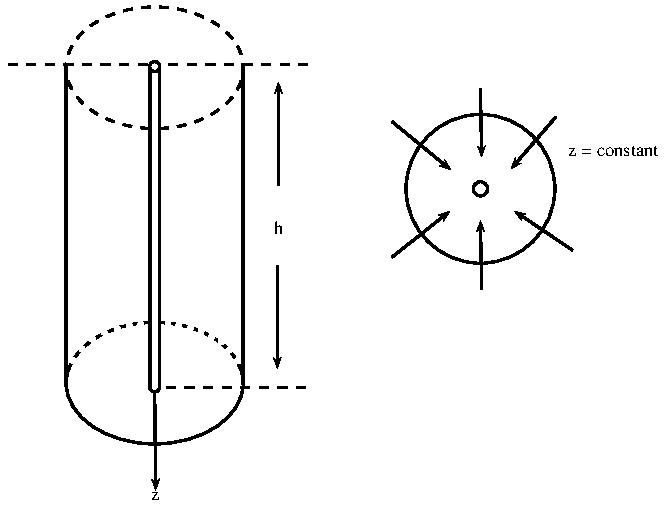
\includegraphics[scale=0.8]{Radial_Flow_Fig.pdf}
        \end{center}
        \caption{Radial flow geometry.}
        \label{Radial_Flow_Fig}
    \end{figure}

    If reservoir is not horizontal, \remove[Murat \c{C}{\i}nar]{our general equation;} Eq. \ref{Continuity_B_ct_Darcy}, applies with $v_{\theta}=0$ and so Eq. \ref{Continuity_B_ct_Darcy} becomes in $r-z$ coordinates.

    \begin{equation}
        \begin{split}
    & \frac{1}{r}\frac{\partial }{\partial r}\left[ \frac{r{{k}_{r}}}{\mu B}\left( \frac{\partial p}{\partial r}-\gamma \frac{\partial z'}{\partial r} \right) \right] \\
    & +\frac{\partial }{\partial z}\left[ \frac{{{k}_{z}}}{\mu B}\left( \frac{\partial p}{\partial z}-\gamma \frac{\partial z'}{\partial z} \right) \right]=\frac{\phi {{c}_{t}}}{B}\frac{\partial p}{\partial t} \\
    \end{split}
        \label{Radial_Flow}
    \end{equation}

    \change[Murat \c{C}{\i}nar]{If we assume}{Now assume} $z=z'$ and $\theta=0$, then $\frac{\partial z'}{\partial r}=0$
    \begin{figure}
        \begin{center}
        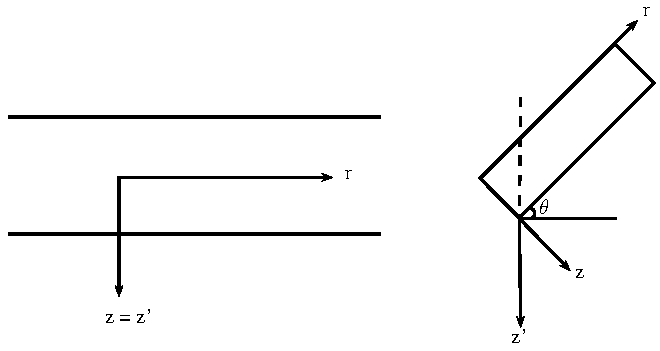
\includegraphics[scale=1]{r_z.pdf}
        \end{center}
        \caption{r-z coordinates.}
        \label{r_z}
    \end{figure}

    For a completely penetrating well, it is physically reasonable to assume $v_{z}\approx0$ ($k_{z}\ll k_{r}$), i.e.,
    \begin{equation}
    \begin{split}
    & {{v}_{z}}=-\frac{{{k}_{z}}}{\mu }\left( \frac{\partial p}{\partial z}-\gamma \frac{\partial z'}{\partial z} \right)=0\quad ;\quad \frac{\partial z'}{\partial z}=1 \\
    & \frac{\partial p}{\partial z}-\gamma =0\quad ;\quad p\left( {{z}_{2}} \right)=p\left( {{z}_{1}} \right)+\gamma \left( {{z}_{2}}-{{z}_{1}} \right)\quad {{z}_{z}}>{{z}_{1}} \\
    \end{split}
    \end{equation}

        Then \remove[Murat \c{C}{\i}nar]{we arrive at}the general radial flow problem \add[Murat \c{C}{\i}nar]{becomes},
    \begin{equation}
        \frac{1}{r}\frac{\partial }{\partial r}\left( r\frac{{{k}_{r}}}{\mu B}\frac{\partial p}{\partial r} \right)=\frac{\phi {{c}_{t}}}{B}\frac{\partial p}{\partial t}
        \label{Radial_flow_general}
    \end{equation}

    where $\phi$, $c_{t}$, $B$, $k_{r}$, and $\mu$ \change[Murat \c{C}{\i}nar]{can be}{are} functions of pressure.

    \change[Murat \c{C}{\i}nar]{Recalling our}{Recall} pseudo-pressure function defined as,

    \begin{equation}
        m\left( p \right)=\int_{{{p}_{b}}}^{p}{\frac{{{k}_{r}}\left( p \right)}{\mu \left( p \right)B\left( p \right)}dp}
        \label{Pseudo_pressure_r}
    \end{equation}

    Using Eq. \ref{Pseudo_pressure_r}, \remove[Murat \c{C}{\i}nar]{we write} Eq. \ref{Radial_flow_general} \add[Murat \c{C}{\i}nar]{is written} as,

    \begin{equation}
        \frac{1}{r}\frac{\partial }{\partial r}\left( r\frac{\partial m\left( p \right)}{\partial r} \right)=\frac{\phi {{c}_{t}}\mu }{{{k}_{r}}}\frac{\partial m\left( p \right)}{\partial t}
        \label{Radial_flow_Pseudo_pressure}
    \end{equation}

    \subsubsection{Dimensionless Variables}
    In well testing \change[Murat \c{C}{\i}nar]{for two reasons, we are using dimensionless variables to prevent our results,}{dimensionless variables are used for two main reasons;}
    \begin{enumerate}[(i)]
        \item minimize number of variables \change[Murat \c{C}{\i}nar]{(find group parameters)}{(by grouping parameters)}
        \item provide general solutions
    \end{enumerate}
    \change[Murat \c{C}{\i}nar]{If we define a dimensionless time}{Dimensionless time is defined as,}

    \begin{equation}
        {{t}_{D}}=\frac{{{k}_{i}}t}{{{\left( \phi {{c}_{t}}\mu  \right)}_{i}}r_{w}^{2}}
        \label{Dimensionless_time}
    \end{equation}
    where subscript "$i$" refers to initial conditions, i.e.,
    \begin{equation*}
        k_{i} = k(p_{i})\,\,\,;\,\,\ \mu_{i}=\mu(p_{i})\,\,\,etc.
    \end{equation*}

    here $p_{i}$ is the initial reservoir pressure (at some datum) and we assume $p_{i}$ is independent of $r$, then

    \begin{equation}
        \frac{\partial m}{\partial t}=\frac{\partial m}{\partial {{t}_{D}}}\frac{\partial {{t}_{D}}}{\partial t}=\frac{\partial m}{\partial {{t}_{D}}}\left( \frac{{{k}_{i}}}{{{\left( \phi {{c}_{t}}\mu  \right)}_{i}}r_{w}^{2}} \right)
        \label{Dimensionless_radial_1}
    \end{equation}

    Using Eq. \ref{Dimensionless_radial_1} in Eq. \ref{Radial_flow_Pseudo_pressure}, and simplifying gives,\Trcknote[Murat \c{C}{\i}nar]{Typo corrected in the following equation}

    \begin{equation}
        r_{w}^{2}\left[ \frac{1}{r}\frac{\partial }{\partial r}\left( r\frac{\partial m\left( p \right)}{\partial r} \right) \right]=\left( \frac{\phi {{c}_{t}}\mu }{k} \right)\left[ \frac{{{k}_{i}}}{{{\left( \phi {{c}_{t}}\mu  \right)}_{i}}} \right]\frac{\partial m}{\partial {{t}_{D}}}
        \label{Dimensionless_radial_2}
    \end{equation}

    \change[Murat \c{C}{\i}nar]{If we}{Now} define,
    \begin{equation}
        {{r}_{D}}=\frac{r}{{{r}_{w}}}
        \label{Dimensionless_lenght}
    \end{equation}

    and \add[Murat \c{C}{\i}nar]{dimensionless diffusivity,}

    \begin{equation}
        {{\eta }_{D}}=\frac{{k}/{\left( \phi {{c}_{t}}\mu  \right)}\;}{{{{k}_{i}}}/{{{\left( \phi {{c}_{t}}\mu  \right)}_{i}}}\;}
        \label{Dimensionless_diffusivity}
    \end{equation}

    then\remove[Murat \c{C}{\i}nar]{we can write} Eq. \ref{Dimensionless_radial_2} \change[Murat \c{C}{\i}nar]{as}{becomes}

    \begin{equation}
        \frac{1}{{{r}_{D}}}\frac{\partial }{\partial {{r}_{D}}}\left( {{r}_{D}}\frac{\partial m\left( p \right)}{\partial {{r}_{D}}} \right)=\frac{1}{{{\eta }_{D}}}\frac{\partial m\left( p \right)}{\partial {{t}_{D}}}
        \label{Dimensionless_radial_3}
    \end{equation}

    If $\frac{1}{{{\eta }_{D}}}=0$, then Eq. \ref{Dimensionless_radial_3} is a linear p.d.e. .

    \change[Murat \c{C}{\i}nar]{If we assume}{Consider} production at a specified rate q; i.e.,
    \begin{figure}
        \begin{center}
        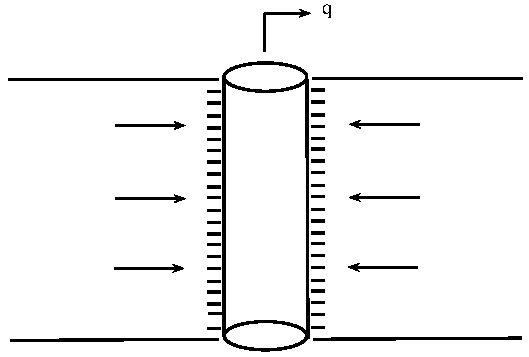
\includegraphics[scale=1]{Production_Full.pdf}
        \end{center}
        \caption{Production from a vertical full penetrating well. Volumetric flux, q, into the wellbore (flow out of the reservoir the boundary represented by wellbore).}
        \label{Production_Full}
    \end{figure}

    Flow rate out = $qB=\int\limits_{S}{\mathbf{v}\,\mathbf{n}\,dS}$ and $\mathbf{n}$ is the unit outward normal to $S$ and is equal to

    \begin{equation*}
        \begin{split}
        & \mathbf{n}=-{{i}_{r}}+0{{i}_{\theta }}+0{{i}_{z}}=\left( 1,0,0 \right) \\
        & \mathbf{v}=\left( {{v}_{r}}+{{v}_{\theta }}+{{v}_{z}} \right) \\
        \end{split}
    \end{equation*}

    \begin{equation*}
        \begin{split}
             qB&=\int\limits_{S}{-{{\left. {{v}_{r}} \right|}_{r={{r}_{w}}}}}dS\quad ;\quad ds={{r}_{w}}d\theta dz \\
             qB&=\int_{0}^{2\pi }{\int_{0}^{h}{{{\left( -{{v}_{r}} \right)}_{{{r}_{w}}}}{{r}_{w}}}}d\theta dz \\
             q&={{\int_{0}^{2\pi }{\int_{0}^{h}{\frac{k}{\mu B}\left( r\frac{\partial p}{\partial r} \right)}}}_{r={{r}_{w}}}}d\theta dz \\
             q&=2\pi {{\int_{0}^{h}{\left( r\frac{\partial m}{\partial r} \right)}}_{{{r}_{w}}}}dz \\
        \end{split}
    \end{equation*}

    \change[Murat \c{C}{\i}nar]{If}{Now} we assume \add[Murat \c{C}{\i}nar]{that} variation of $r\frac{\partial m\left( p \right)}{\partial r}$ in z-direction is insignificant or
    \begin{equation*}
    {{\int\limits_{0}^{h}{\left( r\frac{\partial m\left( p \right)}{\partial r} \right)}}_{{{r}_{w}}}}dz={{\left( r\frac{\partial m\left( p \right)}{\partial r} \right)}_{{{r}_{w}},\widehat{z}}}h
    \end{equation*}
    where $\widehat{z}$ is a mean value between $0\leq \widehat{z} \leq h$. Then the boundary condition is


    \begin{equation}
        q=2\pi h{{\left( r\frac{\partial m\left( p \right)}{\partial r} \right)}_{{{r}_{w}}}}
        \label{Well_boundary}
    \end{equation}

    \change[Murat \c{C}{\i}nar]{If we define}{Define,}
    \begin{equation}
        \begin{split}
         {{m}_{D}}&=\frac{2\pi h\left[ m\left( {{p}_{i}} \right)-m\left( p \right) \right]}{q} \\
        & =\frac{2\pi h}{q}\left[ m\left( {{p}_{i}} \right)-m\left( p \right) \right] \\
        & =\frac{2\pi h}{q}\int\limits_{p}^{{{p}_{i}}}{\frac{k\left( p \right)}{\mu \left( p \right)B\left( p \right)}dp} \\
        \end{split}
        \label{mD_definition}
    \end{equation}

    Then \change[Murat \c{C}{\i}nar]{one}{we} can show that Eqs. \ref{Dimensionless_radial_3} and \ref{Well_boundary}\change[Murat \c{C}{\i}nar]{, respectively, can be}{ is} written as
    \begin{equation}
            \frac{1}{{{r}_{D}}}\frac{\partial }{\partial {{r}_{D}}}\left( {{r}_{D}}\frac{\partial {{m}_{D}}}{\partial {{r}_{D}}} \right)=\frac{1}{{{\eta }_{D}}}\frac{\partial {{m}_{D}}}{\partial {{t}_{D}}}
        \label{Dimensionless_radial_4}
    \end{equation}
    \begin{equation}
            {{\left( {{r}_{D}}\frac{\partial {{m}_{D}}}{\partial {{r}_{D}}} \right)}_{{{r}_{D}}=1}}=-1
        \label{Well_boundary_2}
    \end{equation}
    Note that $r_{D}=1$ corresponds to $r=r_{w}$.
    Initial condition, $p=p_{i}$ at values of $r$ at $\widehat{z}$.
    $m_{D}=0$ at $t_{D}=0$ then,
    \begin{equation}
        {{\left. p\left( r,t \right) \right|}_{t=0}}={{p}_{i}}
        \label{initial_condition}
    \end{equation}

    \change[Murat \c{C}{\i}nar]{Since we consider an infinite reservoir, then}{Infinite acting reservoir is considered implying,}
    \begin{equation*}
        \underset{r\to \omega }{\mathop{\lim }}\,p\left( r,t \right)={{p}_{i}}
    \end{equation*}

    which corresponds to
    \begin{equation}
        \underset{{{r}_{D}}\to \infty }{\mathop{\lim }}\,{{m}_{D}}\left( {{r}_{D}},{{t}_{D}} \right)=0
        \label{initial_condition_md}
    \end{equation}

    In summary, \change[Murat \c{C}{\i}nar]{we have the following IBVP,}{the following initial boundary value problem (IBVP) is achieved with the appropriate boundary conditions.}

    \begin{equation}
        \frac{1}{{{r}_{D}}}\frac{\partial }{\partial {{r}_{D}}}\left( {{r}_{D}}\frac{\partial {{m}_{D}}}{\partial {{r}_{D}}} \right)=\frac{1}{{{\eta }_{D}}}\frac{\partial {{m}_{D}}}{\partial {{t}_{D}}}
        \label{Dimensionless_radial_md_Sum}
    \end{equation}

    \begin{equation}
        {{\left( {{r}_{D}}\frac{\partial {{m}_{D}}}{\partial {{r}_{D}}} \right)}_{{{r}_{D}}=1}}=-1
        \label{Boundary_1_sum}
    \end{equation}

    \begin{equation}
        \underset{{{r}_{D}}\to \infty }{\mathop{\lim }}\,{{m}_{D}}\left( {{r}_{D}},{{t}_{D}} \right)=0
        \label{Boundary_2_sum}
    \end{equation}

    \begin{equation}
        {{m}_{D}}\left( {{r}_{D}},{{t}_{D}}=0 \right)=0
        \label{Initial_con_sum}
    \end{equation}

    Eqs. \ref{Dimensionless_radial_md_Sum}-\ref{Initial_con_sum} lead to give a complete mathematical description of \change[Murat \c{C}{\i}nar]{our}{the} physical problem. Because of ${{\eta }_{D}}$ term, it is a non-linear IBVP. It can also be solved analytically (see Kale and Mattar\cite{Kale_1980_1} or Peres et.al.\cite{Peres_1990_1})

    \change[Murat \c{C}{\i}nar]{Let's now, for}{For} simplicity, assume that variations in $k$, $\phi$, $c_{t}$, and $B$ are small ("negligible") for the pressure change considered. \change[Murat \c{C}{\i}nar]{wit this assumption}{Then,}
     \begin{equation}
        {{\eta }_{D}}=\frac{\left( {k}/{\phi {{c}_{t}}\mu }\; \right)}{{{\left( {k}/{\phi {{c}_{t}}\mu }\; \right)}_{{{p}_{i}}}}}\approx 1
        \label{assumption}
    \end{equation}

    and

    \begin{equation}
        {{\eta }_{D}}=\frac{\left( {k}/{\phi {{c}_{t}}\mu }\; \right)}{{{\left( {k}/{\phi {{c}_{t}}\mu }\; \right)}_{{{p}_{i}}}}}\approx 1
        \label{assumption_1}
    \end{equation}

    \begin{equation}
        m\left( {{p}_{i}} \right)-m\left( p \right)=\int_{p}^{{{p}_{i}}}{\frac{k\left( p \right)}{\mu \left( p \right)B\left( p \right)}dp\approx \frac{{{k}_{i}}}{{{\mu }_{i}}{{B}_{i}}}}\left( {{p}_{i}}-p \right)
        \label{assumption_2}
    \end{equation}

    and then it follows from Eq. \ref{mD_definition} that

    \begin{equation}
        {{m}_{D}}=\frac{2\pi {{k}_{i}} h\left( {{p}_{i}}-p \right)}{q{{B}_{i}}{{\mu }_{i}}}={{p}_{D}}=\frac{2\pi k h\left( {{p}_{i}}-p \right)}{qB\mu }
        \label{mD_to_pD}
    \end{equation}

    \change[Murat \c{C}{\i}nar]{which is the normal}{that is the} definition of dimensionless pressure $p_{D}$ in well testing.
    Considering $\frac{1}{{{\eta }_{D}}}\approx 1$ in Eq. \ref{Dimensionless_radial_md_Sum}, we have

    \begin{equation}
        \frac{1}{{{r}_{D}}}\frac{\partial }{\partial {{r}_{D}}}\left( {{r}_{D}}\frac{\partial {{m}_{D}}}{\partial {{r}_{D}}} \right)=\frac{\partial {{m}_{D}}}{\partial {{t}_{D}}}
        \label{Dimensionless_radial_md_Sum_lin}
    \end{equation}

    \begin{equation}
        {{\left( {{r}_{D}}\frac{\partial {{m}_{D}}}{\partial {{r}_{D}}} \right)}_{{{r}_{D}}=1}}=-1
        \label{Boundary_1_sum_lin}
    \end{equation}

    \begin{equation}
        \underset{{{r}_{D}}\to \infty }{\mathop{\lim }}\,{{m}_{D}}\left( {{r}_{D}},{{t}_{D}} \right)=0
        \label{Boundary_2_sum_lin}
    \end{equation}

    \begin{equation}
        {{m}_{D}}\left( {{r}_{D}},{{t}_{D}}=0 \right)=0
        \label{Initial_con_sum_lin}
    \end{equation}

    Note that Eq. \ref{Dimensionless_radial_md_Sum_lin} is a linear p.d.e. . We seek a solution to the IBVP given by Eqs. \ref{Dimensionless_radial_md_Sum_lin} - \ref{Initial_con_sum_lin}. To find a solution we assume that
    \begin{equation*}
    {{m}_{D}}={{m}_{D}}\left( {{\varepsilon }_{D}} \right)
    \end{equation*}
    where
    \begin{equation*}
    {{\varepsilon }_{D}}=\frac{r_{D}^{2}}{4{{t}_{D}}}={{\varepsilon }_{D}}\left( {{r}_{D}},{{t}_{D}} \right)
    \end{equation*}

    \change[Murat \c{C}{\i}nar]{and can be}{is} called dimensionless Boltzman transform. To use the Boltzman transform, there must be no characteristic length in the system (such as $r_{D}=1$, $r_{w}$). Since the inner boundary condition, Eq. \ref{Boundary_1_sum_lin}, is for a finite wellbore problem, it involves a characteristic length. Thus, to be able to use Boltzman transform, \remove[Murat \c{C}{\i}nar]{we replace} Eq. \ref{Boundary_1_sum_lin} \remove[Murat \c{C}{\i}nar]{is replaced} with one that does not involve characteristic length, \change[Murat \c{C}{\i}nar]{which}{that} is "line source well" inner boundary condition.

    \begin{equation}
        \underset{{{r}_{D}}\to 0}{\mathop{\lim }}\,\left( {{r}_{D}}\frac{\partial {{m}_{D}}}{\partial {{r}_{D}}} \right)=-1
        \label{Line_source_boundary}
    \end{equation}

    Under the preceding assumptions,\remove[Murat \c{C}{\i}nar]{our} approximate problem becomes: Find $m_{D}=m_{D}({\varepsilon }_{D})$ such that $m_{D}$ satisfies

    \begin{equation}
        \frac{1}{{{r}_{D}}}\frac{\partial }{\partial {{r}_{D}}}\left( {{r}_{D}}\frac{\partial {{m}_{D}}}{\partial {{r}_{D}}} \right)=\frac{\partial {{m}_{D}}}{\partial {{t}_{D}}}
        \label{Line_Source}
    \end{equation}

    \begin{equation}
        \underset{{{r}_{D}}\to 0}{\mathop{\lim }}\,\left( {{r}_{D}}\frac{\partial {{m}_{D}}}{\partial {{r}_{D}}} \right)=-1
        \label{Boundary_Line_Source1}
    \end{equation}

    \begin{equation}
        \underset{{{r}_{D}}\to \infty }{\mathop{\lim }}\,{{m}_{D}}\left( {{r}_{D}},{{t}_{D}} \right)=0
        \label{Boundary_Line_Source2}
    \end{equation}

    \begin{equation}
        {{m}_{D}}\left( {{r}_{D}},{{t}_{D}}=0 \right)=0
        \label{Initial_Line_Source}
    \end{equation}

    where,

    \begin{equation}
        {{m}_{D}}=\frac{2\pi h\int_{p}^{{{p}_{i}}}{\frac{k\left( p \right)}{\mu \left( p \right)B\left( p \right)}dp}}{q}
        \label{mD_Line_Source}
    \end{equation}

    Use of Boltzman transformation, ${{\varepsilon }_{D}}=\frac{r_{D}^{2}}{4{{t}_{D}}}$, \change[Murat \c{C}{\i}nar]{will change our}{changes the} p.d.e. to second order ordinary differential equation o.d.e., further \change[Murat \c{C}{\i}nar]{it will collapse our}{collapses} three auxiliary conditions into two conditions,

    \begin{equation}
        \frac{\partial {{m}_{D}}}{\partial {{r}_{D}}}=\frac{\partial {{m}_{D}}}{\partial {{\varepsilon }_{D}}}\frac{\partial {{\varepsilon }_{D}}}{\partial {{r}_{D}}}=\frac{\partial {{m}_{D}}}{\partial {{\varepsilon }_{D}}}\frac{2{{r}_{D}}}{4{{t}_{D}}}
        \label{mD_Boltzman_rD1}
    \end{equation}

    \change[Murat \c{C}{\i}nar]{or}{and}

    \begin{equation}
        {{r}_{D}}\frac{\partial {{m}_{D}}}{\partial {{r}_{D}}}=2\left( \frac{r_{D}^{2}}{4{{t}_{D}}} \right)\frac{d{{m}_{D}}}{d{{\varepsilon }_{D}}}=2{{\varepsilon }_{D}}\frac{d{{m}_{D}}}{d{{\varepsilon }_{D}}}
        \label{mD_Boltzman_rD2}
    \end{equation}

    Using Eq. \ref{mD_Boltzman_rD2} and the chain rule,

        \begin{equation}
        \begin{split}
         \frac{1}{{{r}_{D}}}\frac{\partial }{\partial {{r}_{D}}}\left( {{r}_{D}}\frac{\partial {{m}_{D}}}{\partial {{r}_{D}}} \right)=&\frac{1}{{{r}_{D}}}\frac{d}{d{{\varepsilon }_{D}}}\left( 2{{\varepsilon }_{D}}\frac{d{{m}_{D}}}{d{{\varepsilon }_{D}}} \right)\frac{d{{\varepsilon }_{D}}}{d{{r}_{D}}} \\
        & =\frac{1}{{{t}_{D}}}\frac{d}{d{{\varepsilon }_{D}}}\left( 2{{\varepsilon }_{D}}\frac{d{{m}_{D}}}{d{{\varepsilon }_{D}}} \right) \\
        \end{split}
        \label{mD_Boltzman_rD3}
    \end{equation}

    Similarly,
    \begin{equation}
        \frac{\partial {{m}_{D}}}{\partial {{t}_{D}}}=\frac{d{{m}_{D}}}{d{{\varepsilon }_{D}}}\frac{\partial {{\varepsilon }_{D}}}{\partial {{t}_{D}}}=\frac{d{{m}_{D}}}{d{{\varepsilon }_{D}}}\left( -\frac{r_{D}^{2}}{4t_{D}^{2}} \right)=-\frac{1}{{{t}_{D}}}{{\varepsilon }_{D}}\frac{d{{m}_{D}}}{d{{\varepsilon }_{D}}}
        \label{mD_Boltzman_rD4}
    \end{equation}

    Using Eqs. \ref{mD_Boltzman_rD3} and \ref{mD_Boltzman_rD4} in Eq. \ref{Line_Source} gives,
    \begin{equation}
    {{\varepsilon }_{D}}\frac{d{{m}_{D}}}{d{{\varepsilon }_{D}}}+\frac{d}{d{{\varepsilon }_{D}}}\left( {{\varepsilon }_{D}}\frac{d{{m}_{D}}}{d{{\varepsilon }_{D}}} \right)=0
        \label{mD_Boltzman_Final}
    \end{equation}

    Using Eq. \ref{mD_Boltzman_rD2} \remove[Murat \c{C}{\i}nar]{we can write} the inner boundary condition (see Eq. \ref{Boundary_Line_Source1}) \add[Murat \c{C}{\i}nar]{is written} as

    \begin{equation}
        \underset{{{\varepsilon }_{D}}\to 0}{\mathop{\lim }}\,2{{\varepsilon }_{D}}\frac{d{{m}_{D}}}{d{{\varepsilon }_{D}}}=-1
        \label{line_source_Boltzman_BC}
    \end{equation}


    Initial condition (I.C.) Eq. \ref{Initial_Line_Source},

    \begin{equation*}
        {{t}_{D}}\to 0\quad {{\varepsilon }_{D}}\to \infty \quad \Rightarrow \quad \underset{{{\varepsilon }_{D}}\to \infty }{\mathop{\lim }}\,{{m}_{D}}\left( {{\varepsilon }_{D}} \right)=0
    \end{equation*}

    Outer boundary condition (O.B.C.) Eq. \ref{Boundary_Line_Source2},
    \begin{equation*}
        {{r}_{D}}\to \infty \quad {{\varepsilon }_{D}}\to \infty \quad \Rightarrow \quad \underset{{{\varepsilon }_{D}}\to \infty }{\mathop{\lim }}\,{{m}_{D}}\left( {{\varepsilon }_{D}} \right)=0
    \end{equation*}

    Thus both I.C. and O.B.C. \change[Murat \c{C}{\i}nar]{can be}{is} represented by,

    \begin{equation}
        \underset{{{\varepsilon }_{D}}\to \infty }{\mathop{\lim }}\,{{m}_{D}}\left( {{\varepsilon }_{D}} \right)=0
        \label{line_source_Boltzman_BC2}
    \end{equation}

    We need to solve boundary value problem (B.V.P.) given by Eqs. \ref{mD_Boltzman_Final} - \ref{line_source_Boltzman_BC2}. Let,

    \begin{equation}
        {{w}_{D}}=\frac{d{{m}_{D}}}{d{{\varepsilon }_{D}}}
        \label{wD}
    \end{equation}

    Substituting Eq. \ref{wD} into Eq. \ref{mD_Boltzman_Final} gives,

    \begin{equation*}
        \frac{d}{d{{\varepsilon }_{D}}}\left( {{\varepsilon }_{D}}{{w}_{D}} \right)+{{\varepsilon }_{D}}{{w}_{D}}=0
    \end{equation*}

    \begin{equation*}
        {{\varepsilon }_{D}}\frac{d{{w}_{D}}}{d{{\varepsilon }_{D}}}+{{w}_{D}}+{{\varepsilon }_{D}}{{w}_{D}}=0
    \end{equation*}

    \begin{equation}
        {{\varepsilon }_{D}}\frac{d{{w}_{D}}}{d{{\varepsilon }_{D}}}+\left( 1+{{\varepsilon }_{D}} \right){{w}_{D}}=0
        \label{Sol_wD}
    \end{equation}

    Eq. \ref{Sol_wD} is separable ordinary differential equation, thus separating variables, \remove[Murat \c{C}{\i}nar]{we have}

    \begin{equation}
        \frac{d{{w}_{D}}}{{{w}_{D}}}=-\frac{1+{{\varepsilon }_{D}}}{{{\varepsilon }_{D}}}
        \label{Sol_wD_1}
    \end{equation}

    Interpreting both sides \add[Murat \c{C}{\i}nar]{yields},

    \begin{equation*}
    \ln {{w}_{D}}=-{{\varepsilon }_{D}}-\ln {{\varepsilon }_{D}}+{{c}_{1}}\quad ;\quad {{c}_{1}}\text{ is an integrating constant}
    \end{equation*}

    or

    \begin{equation*}
    \begin{split}
      \ln {{w}_{D}}&=-{{\varepsilon }_{D}}-\ln {{\varepsilon }_{D}}+{{c}_{1}}\quad ;\quad {{c}_{1}}\text{ is an integrating constant} \\
     {{w}_{D}}&=\exp \left[ -{{\varepsilon }_{D}}-\ln {{\varepsilon }_{D}}+{{c}_{1}} \right] \\
    & ={{e}^{{{c}_{1}}}}\frac{1}{{{\varepsilon }_{D}}}{{e}^{-{{\varepsilon }_{D}}}}=\frac{c}{{{\varepsilon }_{D}}}{{e}^{-{{\varepsilon }_{D}}}}\quad ;\quad c={{e}^{{{c}_{1}}}} \\
    \end{split}
    \end{equation*}

    At this point, we have

    \begin{equation*}
        {{w}_{D}}=\frac{d{{m}_{D}}}{d{{\varepsilon }_{D}}}=\frac{c}{{{\varepsilon }_{D}}}\exp \left[ -{{\varepsilon }_{D}} \right]
    \end{equation*}

    thus

    \begin{equation}
        2{{\varepsilon }_{D}}\frac{d{{m}_{D}}}{d{{\varepsilon }_{D}}}=2c\exp \left[ -{{\varepsilon }_{D}} \right]
        \label{Sol_wD_2}
    \end{equation}

    It follows from Eq. \ref{line_source_Boltzman_BC} and \ref{Sol_wD_2} that

    \begin{equation}
        c=-1/2
        \label{Sol_wD_3}
    \end{equation}

    Thus Eq. \ref{Sol_wD_2} becomes

    \begin{equation}
        \frac{d{{m}_{D}}}{d{{\varepsilon }_{D}}}=-\frac{1}{2{{\varepsilon }_{D}}}\exp \left[ -{{\varepsilon }_{D}} \right]
        \label{Sol_wD_4}
    \end{equation}

    Integrating Eq. \ref{Sol_wD_4} from ${\varepsilon }_{D}$ to $\infty$ gives,

    \begin{equation*}
       \int_{{{\varepsilon }_{D}}}^{\infty }{\frac{d{{m}_{D}}}{d{{\varepsilon }_{D}}}}\,d{{\varepsilon }_{D}}=-\frac{1}{2}\int_{{{t}_{D}}}^{\infty }{\frac{\exp \left[ -u \right]}{u}}\,du
    \end{equation*}

    in limit

    \begin{equation}
        \underset{{{\varepsilon }_{D}}\to \infty }{\mathop{\lim }}\,{{m}_{D}}\left( {{\varepsilon }_{D}} \right)-{{m}_{D}}\left( {{\varepsilon }_{D}} \right)=-\frac{1}{2}\int_{{{t}_{D}}}^{\infty }{\frac{\exp \left[ -u \right]}{u}}\,du
        \label{Sol_wD_5}
    \end{equation}

    It follows from Eq. \ref{line_source_Boltzman_BC2} and \ref{Sol_wD_5} that

    \begin{equation}
       {{  m }_{D}}\left( {{\varepsilon }_{D}} \right)=\frac{1}{2}\int_{\frac{t_{D}^{2}}{4{{t}_{D}}}}^{\infty }{\frac{{{\operatorname{e}}^{-u}}}{u}}\,du
        \label{Theis_Solution}
    \end{equation}

    which is known as the Theis solution \cite{Theis_1935_1}. Eq. \ref{Theis_Solution} is also referred to as the line source or the exponential integral or $E_{i}$ solution.

    \change[Murat \c{C}{\i}nar]{In the literature, we use the definition given by,}{Exponential integral is defined by}

    \begin{equation*}
        -{{E}_{i}}\left[ -x \right]=\int_{x}^{\infty }{\frac{{{\operatorname{e}}^{-u}}}{u}}\,du\quad ;\quad {{E}_{i}}\text{ function}
    \end{equation*}

    Exponential integral function is also referred to as $E_[1](x)$,

    \begin{equation}
        -{{E}_{i}}\left[ -x \right]={{E}_{1}}\left( x \right)
        \label{Ei_E1}
    \end{equation}

    with this notation \remove[Murat \c{C}{\i}nar]{we can write} Eq. \ref{Theis_Solution} \change[Murat \c{C}{\i}nar]{as}{becomes}

    \begin{equation}
        {{ m }_{D}}\left( {{\varepsilon }_{D}} \right)=-{{E}_{i}}\left[ -\frac{r_{D}^{2}}{4{{t}_{D}}} \right]
        \label{Theis_Solution_Ei}
    \end{equation}

    The series expansion of $E_{i}$ function \cite{Abramowitz_1965_1}

    \begin{equation}
        {{E}_{i}}\left[ -x \right]=\widetilde{\gamma }+\ln x+\sum\limits_{n=1}^{\infty }{\frac{{{x}^{n}}}{nn!}}
        \label{Ei_expansion}
    \end{equation}

    \change[Murat \c{C}{\i}nar]{If we let}{Let} $x\rightarrow0$ in Eq. \ref{Theis_Solution_Ei}, then we obtain

    \begin{equation}
        \underset{x\to 0}{\mathop{\lim }}\,{{E}_{i}}\left[ -x \right]=\widetilde{\gamma }+\ln x
        \label{Ei_approx}
    \end{equation}

    where $\widetilde{\gamma }$ is \remove[Murat \c{C}{\i}nar]{referred to as} Euler's constant and defined by,

    \begin{equation}
        \widetilde{\gamma }=\underset{n\to \infty }{\mathop{\lim \left\{ \sum\limits_{k=1}^{n}{\frac{1}{k}-\ln \left( n \right)} \right\}}}\,=0.5772156649...
        \label{Eulers_constant}
    \end{equation}

    If we consider that $\frac{r_{D}^{2}}{4{{t}_{D}}}$ is sufficiently small so that \remove[Murat \c{C}{\i}nar]{we can approximate} ${{E}_{i}}\left[ -\frac{r_{D}^{2}}{4{{t}_{D}}} \right]$ \add[Murat \c{C}{\i}nar]{is approximated} by\remove[Murat \c{C}{\i}nar]{the right hand side of} Eq. \ref{Ei_approx}. Then, Eq. \ref{Theis_Solution_Ei} \change[Murat \c{C}{\i}nar]{can be}{is} approximated as

    \begin{equation}
        {{ m }_{D}}\left( {{\varepsilon }_{D}} \right)=-\frac{1}{2}\left[ \ln \left( \frac{r_{D}^{2}}{4{{t}_{D}}} \right)+\widetilde{\gamma } \right]
        \label{Semilog_Approx1}
    \end{equation}

    or

    \begin{equation}
        {{ m }_{D}}=\frac{1}{2}\ln \left( \frac{4{{t}_{D}}}{r_{D}^{2}{{e}^{\widetilde{\gamma }}}} \right)
        \label{Semilog_Approx2}
    \end{equation}

    which is referred to as the semilog approximation to Eq. \ref{Theis_Solution_Ei}.

    Although \remove[Murat \c{C}{\i}nar]{we derived}Eq. \ref{Semilog_Approx2} \add[Murat \c{C}{\i}nar]{is derived} as a limiting form of Eq. \ref{Theis_Solution_Ei} as $\frac{r_{D}^{2}}{4{{t}_{D}}}\to 0$, Eq. \ref{Theis_Solution_Ei} \change[Murat \c{C}{\i}nar]{can also be}{is} well approximated by Eq. \ref{Semilog_Approx2} if

    \begin{equation*}
        \frac{r_{D}^{2}}{4{{t}_{D}}}\le \frac{1}{100}
    \end{equation*}

    which is equivalent to;

    \begin{equation}
        \frac{{{t}_{D}}}{r_{D}^{2}}\ge 25
        \label{Semilog_Approx2_}
    \end{equation}

    \begin{figure}
        \begin{center}
        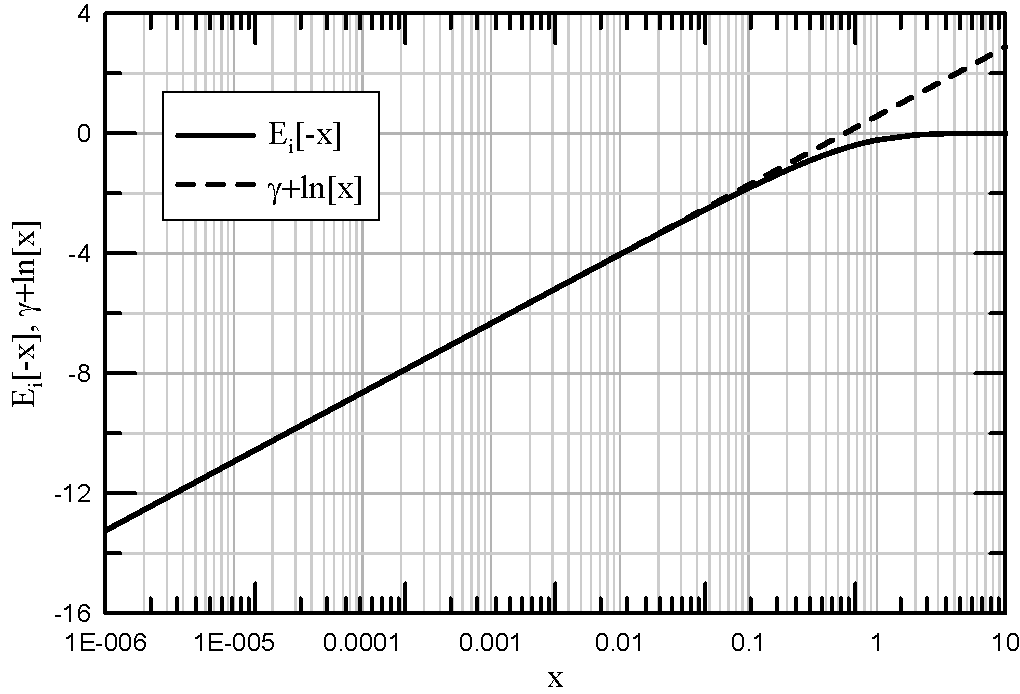
\includegraphics[scale=0.7]{Exponential_Integral_approximation.pdf}
        \end{center}
        \caption{Comparison of exponential integral with logarithmic approximation given by Eq. \ref{Ei_approx}.}
        \label{Exponential_Integral_approximation}
    \end{figure}

    \vspace{15pt}
    \large{\textbf{Remark on exponential integral approximation:}}\\
    \rule{\textwidth}{1pt}
     At $r=r_{w}$, $r_{D}=r/r_{w}=1$ and Eq. \ref{Semilog_Approx2} becomes,
    \begin{equation*}
        \frac{2.637\times {{10}^{-3}}{{k}_{i}}t}{{{\left( \phi \mu {{c}_{t}} \right)}_{i}}r_{w}^{2}}\ge 25
    \end{equation*}

    where $t$ is in hrs. \change[Murat \c{C}{\i}nar]{Let's}{Now} suppose,
    $r_{w}=0.35$ ft, $\mu_{i}=0.8$ cp, $\phi_{i}=0.1$, $k_{i}=10$ md, and $c_{t}=1.1\times10^{5}$.
    then it follows that

    \begin{equation*}
        t_{D}\approx2.5\times10^{5}t
    \end{equation*}

    In order for Eq. \ref{Ei_approx} to hold, we need

    \begin{equation*}
        2.5\times10^{5}t\geq25\quad\Rightarrow\quad t\geq1.0\times10^{-4}hrs(=0.36seconds)
    \end{equation*}

    This \add[Murat \c{C}{\i}nar]{example} illustrates that at the wellbore $(r_{D}=1)$, the semilog approximation of the line source solution becomes valid within several seconds to a very few minutes for reasonable values of\remove[Murat \c{C}{\i}nar]{the} physical parameters; (e.g. $k_{i}$, $c_{t}$...). If \remove[Murat \c{C}{\i}nar]{we are using} the semilog approximation of the line source \add[Murat \c{C}{\i}nar]{solution is used} to analyze \remove[Murat \c{C}{\i}nar]{the} interference data with \change[Murat \c{C}{\i}nar]{the}{an} observation well say at $r=1000r_{w}$, ($r_{D}=1000$) \add[Murat \c{C}{\i}nar]{away} from \change[Murat \c{C}{\i}nar]{the}{a} flowing well, then for the values of physical parameters considered, Eq. \ref{Semilog_Approx2_} requires,

    \begin{equation*}
        t\geq10^{-4}{r_{D}^{2}}=100 hrs
    \end{equation*}

    In short, \remove[Murat \c{C}{\i}nar]{we can use }the semilog approximation of the line source solution \add[Murat \c{C}{\i}nar]{is used}, i.e., Eq. \ref{Ei_approx} to analyze well test pressure data measured either at the active (producing) well or at the observation (shut-in) well provided that test time satisfies Eq. \ref{Semilog_Approx2_}.\\
    \rule{\textwidth}{1pt}\\
    \vspace{15pt}

    \change[Murat \c{C}{\i}nar]{To obtain the line source solution which is given by}{Line source solution given by} Eq. \ref{Line_Source} \change[Murat \c{C}{\i}nar]{is obtained by using the line source boundary condition}{we used the line source well boundary condition} Eq. \ref{Line_source_boundary} that is
    \begin{equation*}
    \underset{{{r}_{D}}\to 0}{\mathop{\lim }}\,\left( {{r}_{D}}\frac{\partial {{m}_{D}}}{\partial {{r}_{D}}} \right)=-1
    \end{equation*}

    Differentiating Eq. \ref{Line_Source} with respect to $r_{D}$ gives,
    \begin{equation}
    \frac{\partial {{ m }_{D}}}{\partial {{r}_{D}}}=\frac{1}{2}\frac{\partial }{\partial {{r}_{D}}}\left[ \int_{\frac{t_{D}^{2}}{4{{t}_{D}}}}^{\infty }{\frac{{{\operatorname{e}}^{-u}}}{u}}\,du \right]=-\frac{1}{2}\frac{\partial }{\partial {{r}_{D}}}\left[ \int_{\infty }^{\frac{t_{D}^{2}}{4{{t}_{D}}}}{\frac{{{\operatorname{e}}^{-u}}}{u}}\,du \right]
        \label{Line_Solution_dif_rD}
    \end{equation}

    \change[Murat \c{C}{\i}nar]{From calculus we know that}{Recall,}

    \begin{equation}
    \frac{d}{dx}\left[ \int_{a}^{b\left( x \right)}{f\left( z \right)dz} \right]=f\left[ b\left( x \right) \right]\frac{db\left( x \right)}{dx}
        \label{Calculus_1}
    \end{equation}

    where $a$ is \add[Murat \c{C}{\i}nar]{a}constant. Using the formula given by Eq. \ref{Calculus_1} in Eq. \ref{Line_Solution_dif_rD} and simplifying the resulting equation; \remove[Murat \c{C}{\i}nar]{we obtain}

    \begin{equation}
    \frac{\partial {{ m }_{D}}}{\partial {{r}_{D}}}=-\frac{1}{{{r}_{D}}}\exp \left[ -\frac{r_{D}^{2}}{4{{t}_{D}}} \right]
        \label{Boundary_der1}
    \end{equation}

    Multiplying Eq. \ref{Boundary_der1} by $r_{D}$

    \begin{equation}
    {{r}_{D}}\frac{\partial {{ m }_{D}}}{\partial {{r}_{D}}}=-\exp \left[ -\frac{r_{D}^{2}}{4{{t}_{D}}} \right]
        \label{Boundary_der2}
    \end{equation}

    \change[Murat \c{C}{\i}nar]{so as expected our}{Thus the} line source solution satisfies \remove[Murat \c{C}{\i}nar]{our} line source wellbore B.C., i.e.,

    \begin{equation*}
        \underset{{{r}_{D}}\to 0}{\mathop{\lim }}\,\left( {{r}_{D}}\frac{\partial {{m}_{D}}}{\partial {{r}_{D}}} \right)=-1
    \end{equation*}

    It is important to note that Eq. \ref{Line_Source} assumes \remove[Murat \c{C}{\i}nar]{that we have} a well with vanishingly small radius\change[Murat \c{C}{\i}nar]{. However the more}{,however, the more} rigorous solution \change[Murat \c{C}{\i}nar]{will be}{is} the one considering \change[Murat \c{C}{\i}nar]{the}{a} well with finite wellbore. To obtain a solution for a well with finite wellbore producing at a constant rate,\remove[Murat \c{C}{\i}nar]{we need to use} an inner boundary condition \remove[Murat \c{C}{\i}nar]{is used} such that

    \begin{equation}
        \underset{{{r}_{D}}\to 0}{\mathop{\lim }}\,\left( {{r}_{D}}\frac{\partial {{m}_{D}}}{\partial {{r}_{D}}} \right)=-1
        \label{Inner_Boundary1}
    \end{equation}

    Therefore, the finite wellbore radius I.B.V.P. differs from the line source I.B.V.P. in \change[Murat \c{C}{\i}nar]{that our}{the} boundary condition \remove[Murat \c{C}{\i}nar]{is} given by Eq. \ref{Inner_Boundary1}\change[Murat \c{C}{\i}nar]{ instead of}{Line source solution is closed with} Eq. \ref{Line_source_boundary}.

    Note that $r_{D}=1$ (see Eq. \ref{Line_Solution_dif_rD}), the line source solution satisfies

    \begin{equation}
        {{\left( {{r}_{D}}\frac{\partial {{ m }_{D}}}{\partial {{r}_{D}}} \right)}_{{{r}_{D}}=1}}=-\exp \left[ -\frac{1}{4{{t}_{D}}} \right]
        \label{Boundary_der3}
    \end{equation}

    As $t_{D}\rightarrow\infty$, the RHS of Eq. \ref{Boundary_der3} approaches $-1$, i.e.,

    \begin{equation}
    \underset{{{t}_{D}}\to \infty }{\mathop{\lim }}\,{{\left( {{r}_{D}}\frac{\partial {{ m }_{D}}}{\partial {{r}_{D}}} \right)}_{{{r}_{D}}=1}}=-1
        \label{Boundary_der4}
    \end{equation}

    from which intuitively we expect that at sufficiently large\remove[Murat \c{C}{\i}nar]{ values of} times, the line source solution \change[Murat \c{C}{\i}nar]{(for $r_{D}\geq1$)}{for $r_{D}=1$} will be very close to the finite wellbore radius solution. In fact for $t_{D}>25$, the RHS of Eq. \ref{Boundary_der3} is within $1\%$ of $-1$.

    Mueller and Witherspoon \cite{Mueller_1965_1} were the ones first to investigate the validity of line source solution. They compared the finite wellbore radius solution and the line source solution. Such comparison is shown in Fig. \ref{Line_Finite_Comp} \change[Murat \c{C}{\i}nar]{which is taken from Earlougher's manograph, SPE Monograph 5. It is a}{- log-log plot of $p_{D} (=m_{D})$ versus $t_{D}/r_{D}^{2}$}.

    \begin{figure}
        \begin{center}
        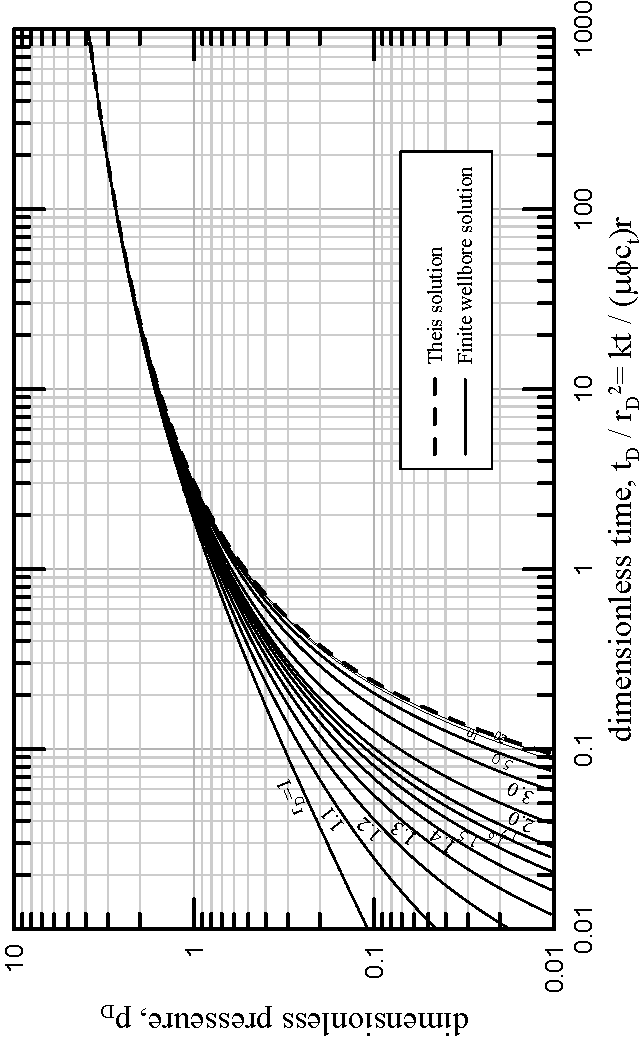
\includegraphics[scale=1]{Line_Finite_Comp.pdf}
        \end{center}
        \caption{Comparison of line source solution to finite radius wellbore solution\cite{Mueller_1965_1}.}
        \label{Line_Finite_Comp}
    \end{figure}

    The dashed curve in the figure represents the exponential integral solution(or the line source solution) given by Eq. \ref{Line_Source}. The top solid curve corresponds to the finite wellbore radius solution evaluated at the wellbore (i.e. $r_D=1$). All other solid curves represent finite wellbore radius solution at various locations (different $r_{D}$ values) in the reservoir.

    \change[Murat \c{C}{\i}nar]{From the figure we see that if}{Figure indicates that when} $t_{D}/r_{D}^{2}\geq25$, the difference between the finite wellbore radius solution and the line source solution is negligible. \change[Murat \c{C}{\i}nar]{This means that}{Thus} at $r_{D}=1$ (at the wellbore) \remove[Murat \c{C}{\i}nar]{we need} $t_{D}\geq25$ \add[Murat \c{C}{\i}nar]{is required} for \remove[Murat \c{C}{\i}nar]{the} two solutions to be essentially the same. Also note that if $r_{D}\geq20$, then the two solutions are essentially equal for all values of the dimensionless time $t_{D}$ of practical interest.\\

    For the interference testing purposes, the difference between the line source solution and the finite wellbore radius solution is negligible.
    To use Eq. \ref{Line_Source} for the analysis of pressure data measured at a flowing well, we evaluate Eq. \ref{Line_Source} at $r_{D}=1$ and use the notation

    \begin{equation}
           p\left( {{r}_{D}}=1,{{t}_{D}} \right)=p\left( r={{r}_{w}},t \right)={{p}_{wf}}={{p}_{wf}}\left( t \right)
        \label{Pwf}
    \end{equation}

    \subsection{Semilog analysis}

    \change[Murat \c{C}{\i}nar]{From our previous derivations}{In the previous section,} we showed that if $t_{D}/r_{D}^{2}\geq25$, the semilog approximation of the line source solution is given by Eq. \ref{Semilog_Approx2} i.e.;

    \begin{equation*}
        {{ m }_{D}}=\frac{1}{2}\ln \left( \frac{4{{t}_{D}}}{r_{D}^{2}{{e}^{\widetilde{\gamma }}}} \right)
    \end{equation*}

    At $r_{D}=1$, \remove[Murat \c{C}{\i}nar]{that gives,}

    \begin{equation}
        \begin{split}
     {{m}_{D}}\left( {{r}_{D}}=1 \right)&=\frac{2\pi h}{q}\int_{{{p}_{wf}}}^{{{p}_{i}}}{\frac{k\left( p \right)}{\mu \left( p \right)B\left( p \right)}}\,dp \\
    & =\frac{1}{2}\left[ \frac{4{{t}_{D}}}{{{e}^{\widetilde{\gamma }}}} \right] \\
    & =\frac{1}{2}\left( \ln {{t}_{D}}+0.80907 \right) \\
    \end{split}
        \label{mpwf_1}
    \end{equation}

    or

    \begin{equation}
       \begin{split}
        & {{m}_{D}}\left( {{r}_{D}}=1 \right)=\underbrace{\frac{1}{2\log \left( e \right)}}_{\text{1}\text{.15129}} \\
    & \left\{ \log \left( t \right)+\log \left[ \frac{{{k}_{i}}}{{{\left( \phi {{c}_{t}}\mu  \right)}_{i}}r_{w}^{2}} \right]+\underbrace{\log \left( e \right)\ln \left( \frac{4}{{{e}^{\widetilde{\gamma }}}} \right)}_{\text{0}\text{.351378}} \right\} \\
    \end{split}
        \label{mpwf_2}
    \end{equation}

    Note that

    \begin{equation}
     \begin{split}
     {{m}_{D}}\left( {{r}_{D}}=1 \right)&=\frac{2\pi h}{q}\int_{{{p}_{wf}}}^{{{p}_{i}}}{\frac{k\left( p \right)}{\mu \left( p \right)B\left( p \right)}}dp \\
     & =\frac{2\pi h}{q}\left[ m\left( {{p}_{i}} \right)-m\left( {{p}_{wf}} \right) \right] \\
    \end{split}
        \label{mpwf_3}
    \end{equation}

    Then it follows from Eq. \ref{mpwf_2} and \ref{mpwf_3} that

    \begin{equation}
    \begin{split}
    & m\left( {{p}_{wf}} \right)=m\left( {{p}_{i}} \right)-\text{1}\text{.15129}\frac{q}{2\pi h} \\
    & \left\{ \log \left( t \right)+\log \left[ \frac{{{k}_{i}}}{{{\left( \phi {{c}_{t}}\mu  \right)}_{i}}r_{w}^{2}} \right]+\text{0}\text{.351378} \right\} \\
    \end{split}
        \label{mpwf_4}
    \end{equation}

    which indicates that a semilog plot of $m(p_{wf})$ versus $t$ \change[Murat \c{C}{\i}nar]{which}{that} yields a straight line \change[Murat \c{C}{\i}nar]{of}{with a} slope

    \begin{equation}
        \text{slope}=\widetilde{m}=-\text{1}\text{.15129}\frac{q}{2\pi h}
        \label{semilog_slope}
    \end{equation}

    \change[Murat \c{C}{\i}nar]{from which we can compute $h$}{$h$ is computed from the slope of semilog straight line.}
    \change[Murat \c{C}{\i}nar]{Suppose we}{Now} differentiate Eq. \ref{mpwf_2} w.r.t. $logt$.

    \begin{equation}
    \frac{2\pi h}{q}\frac{d}{d\log }\int_{{{p}_{wf}}}^{{{p}_{i}}}{\frac{k\left( p \right)}{\mu \left( p \right)B\left( p \right)}}dp=1.15129
        \label{semilog_slope_1}
    \end{equation}

    or

    \begin{equation*}
        \frac{2\pi h}{q}\frac{d}{d{{p}_{wf}}}\left\{ \int_{{{p}_{wf}}}^{{{p}_{i}}}{\frac{k\left( p \right)}{\mu \left( p \right)B\left( p \right)}}dp \right\}\frac{d{{p}_{wf}}}{d\log t}=1.15129
    \end{equation*}

    or

    \begin{equation*}
        \frac{2\pi h}{q}\left[ -\frac{k\left( {{p}_{wf}} \right)}{\mu \left( {{p}_{wf}} \right)B\left( {{p}_{wf}} \right)} \right]\frac{d{{p}_{wf}}}{d\log t}=1.15129
    \end{equation*}

    or

    \begin{equation}
        \frac{k\left( {{p}_{wf}} \right)}{\mu \left( {{p}_{wf}} \right)B\left( {{p}_{wf}} \right)}=-\text{1}\text{.15129}\frac{q}{2\pi h\left( d{{p}_{wf}}/d\log t \right)}
        \label{semilog_slope2}
    \end{equation}

    \vspace{15pt}
    \large{\textbf{Aside:}}\\
    \rule{\textwidth}{1pt}
    For solution gas drive reservoirs, B${\o}$e et.al.\cite{Boe_1989_1}  showed that pressure and oil saturation, $S_{o}$ are unique function of the Boltzman variable $r_{D}^{2}/4t_{D}$, or $r^{2}/t$ provided that $t_{D}/r_{D}^{2}\geq25$.

    Serra et. al. \cite{Serra_1990_1} used this observation to show how to compute effective permeability from wellbore B.C. for constant oil rate.

    \begin{equation}
        {{q}_{o}}=2\pi {{\left( \frac{k{{k}_{ro}}}{{{\mu }_{o}}}rh\frac{\partial p}{\partial r} \right)}_{r={{r}_{w}}}}
        \label{q_rw}
    \end{equation}

    Suppose $p$ is a function of the Boltzman variable $z=r^{2}/t$ then,

    \begin{equation}
        \frac{\partial p}{\partial r}=\frac{dp}{dz}\frac{dz}{dr}=\frac{dp}{dz}\frac{2r}{t}
        \label{chain_dpdr_z}
    \end{equation}

    and
    \begin{equation}
        \frac{\partial p}{\partial t}=\frac{dp}{dz}\frac{dz}{dt}=\frac{dp}{dz}\left( -\frac{{{r}^{2}}}{{{t}^{2}}} \right)
        \label{chain_dpdt_z}
    \end{equation}

    It follows that

    \begin{equation*}
    r\frac{\partial p}{\partial r}=2\frac{{{r}^{2}}}{t}\frac{dp}{dz}=\left( -2t \right)\frac{-{{r}^{2}}}{{{t}^{2}}}=-2t\frac{dp}{dt}=-2\frac{dp}{d\ln t}
    \end{equation*}

    or at $r=r_{w}$

    \begin{equation}
    {{\left( r\frac{\partial p}{\partial r} \right)}_{{{r}_{w}}}}=-2t\frac{d{{p}_{wf}}}{dt}=-2\frac{d{{p}_{wf}}}{d\ln t}
        \label{dpwf_dlnt}
    \end{equation}

    Using Eq. \ref{q_rw} in Eq. \ref{dpwf_dlnt} gives,

    \begin{equation}
    {{q}_{o}}=2\pi h{{\left( \frac{k{{k}_{ro}}}{{{\mu }_{o}}{{B}_{o}}} \right)}_{{{r}_{w}}}}\left( -2\frac{d{{p}_{wf}}}{d\ln t} \right)
        \label{q_rw_2}
    \end{equation}

    Rearranging Eq. \ref{q_rw_2}, we obtain,

    \begin{equation}
    {{\left( \frac{k{{k}_{ro}}}{{{\mu }_{o}}{{B}_{o}}} \right)}_{{{r}_{w}}}}=-\frac{{{q}_{o}}}{4\pi h\left( \frac{d{{p}_{wf}}}{d\ln t} \right)}
        \label{q_rw_3}
    \end{equation}

   \change[Murat \c{C}{\i}nar]{which gives us a way for}{that provides a way of} computing ${{\left( k{{k}_{ro}} \right)}_{{{p}_{wf}}}}$ as a function of $p_{wf}$ from

    \begin{equation}
        \begin{split}
     {{\left( k{{k}_{ro}} \right)}_{{{p}_{wf}}}}&=-\frac{{{q}_{o}}{{\left( {{\mu }_{o}}{{B}_{o}} \right)}_{{{p}_{wf}}}}}{4\pi h\left( \frac{d{{p}_{wf}}}{d\ln t} \right)} \\
    & =-\frac{2.303{{q}_{o}}{{\left( {{\mu }_{o}}{{B}_{o}} \right)}_{{{p}_{wf}}}}}{4\pi h\left( \frac{d{{p}_{wf}}}{d\log t} \right)}\quad ;\quad \ln t=2.303\log t \\
    \end{split}
        \label{kkro_compute}
    \end{equation}

    Eq. \ref{kkro_compute} implies that $k_{ro}$ is a function of pressure. \remove[Murat \c{C}{\i}nar]{This means, we must be able to consider $S_{o}=S_{o}(p)$ i.e. oil saturation is a function of pressure.}{Therefore, oil saturation is considered as a function of pressure, i.e. $S_{o}=S_{o}(p)$ .} \remove[Murat \c{C}{\i}nar]{Aanonsen (PhD, 1985) derived a relation to obtain $S_{o}$ as afunction of pressure. Then we can construct $k_{ro} versus S_{o}$.}\\
    \rule{\textwidth}{1pt}\\
    \vspace{15pt}

    \change[Murat \c{C}{\i}nar]{if we now concentrate on}{Now we consider} the case when the variations in $k(p)$, $\mu(p)$,and $B(p)$ are negligible,

    \begin{equation}
        {{m}_{D}}={{p}_{D}}=\frac{2\pi kh\left[ {{p}_{i}}-p\left( r,t \right) \right]}{qB\mu }
        \label{mD_no_p_var}
    \end{equation}

    \begin{equation}
        {{t}_{D}}=\frac{kt}{\phi {{c}_{t}}\mu r_{w}^{2}}
        \label{tD_no_p_var}
    \end{equation}

    Suppose that \remove[Murat \c{C}{\i}nar]{we measured the }pressure at any point $r\neq r_{w}$ in the reservoir \add[Murat \c{C}{\i}nar]{is measured}. \change[Murat \c{C}{\i}nar]{When}{If} the semilog approximation to the line source holds, it follows that

    \begin{equation}
        {{p}_{D}}=\frac{1}{2}\ln \left[ \frac{4{{t}_{D}}}{{{e}^{\widetilde{\gamma }}}r_{D}^{2}} \right]
        \label{pD_no_p_var_rD}
    \end{equation}

    or using the dimensional variables \remove[Murat \c{C}{\i}nar]{we obtain}

    \begin{equation}
        \begin{split}
        & p\left( r,t \right)={{p}_{i}}-1.15129\frac{qB\mu }{2\pi kh} \\
        & \left\{ \log \left( t \right)+\log \left[ \frac{{{k}h}}{\phi {{c}_{t}}h\mu r^{2}} \right]+0.351378 \right\} \\
        \end{split}
        \label{p_r_t}
    \end{equation}

    which also indicates that a semilog plot of $p$ versus $t$ \change[Murat \c{C}{\i}nar]{will give us}{gives} a straight line with a slope equal to
    \begin{equation}
    \widetilde{m}=-1.15129\frac{qB\mu }{2\pi kh}\Rightarrow kh=-1.15129\frac{qB\mu }{2\pi \widetilde{m}}
        \label{slope_p_r_t}
    \end{equation}

    Note that \change[Murat \c{C}{\i}nar]{we could also plot the pressure drop}{the pressure drop could also be plotted} as a function of $t$, i.e., $\Delta p\left( r,t \right)={{p}_{i}}-p\left( r,t \right)$. In this case, a semilog plot of $\Delta p$ versus $t$ yields a semilog slope of

    \begin{equation}
    \widetilde{m}=1.15129\frac{qB\mu }{2\pi kh}\quad ; \quad \widetilde{m}\geq 0
        \label{slope_dp_r_t}
    \end{equation}

    \begin{figure}
        \begin{center}
        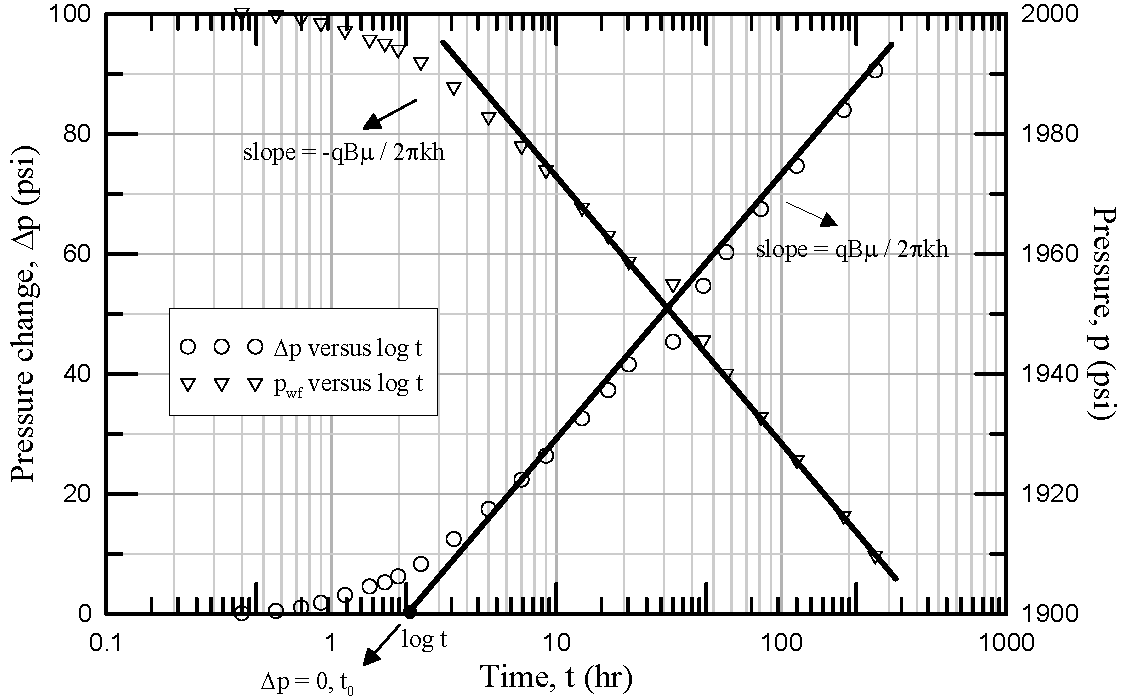
\includegraphics[scale=0.6]{Semilog_dp_vs_p.pdf}
        \end{center}
        \caption{Semilog analysis.}
        \label{Semilog_dp_vs_p}
    \end{figure}

    If we extrapolate the semilog straight line to zero pressure drop in a plot of $\Delta p$ versus $log t$ and denote time time at which $\Delta p=0$ as $t_{0}$ then it follows from Eq. \ref{p_r_t} that

    \begin{equation}
    \begin{split}
     & \Delta p{{\left( r,t \right)}_{t={{t}_{0}}}}=\text{1}\text{.15129}\frac{qB\mu }{2\pi kh} \\
    & \left\{ \log \left( {{t}_{0}} \right)+\log \left[ \frac{kh}{\phi {{c}_{t}}h\mu {{r}^{2}}} \right]+\text{0}\text{.351378} \right\}=0 \\
    \end{split}
        \label{slope_dp_r_t0}
    \end{equation}

    then,

    \begin{equation*}
        \log \left( {{t}_{0}} \right)=-\log \left[ \frac{kh}{\phi {{c}_{t}}h\mu {{r}^{2}}} \right]-0.351378
    \end{equation*}

    or

    \begin{equation}
        \log \left( {{t}_{0}} \right)=-\log \left[ \frac{kh}{\phi {{c}_{t}}h\mu {{r}^{2}}}{{10}^{0.351378}} \right]
        \label{t0}
    \end{equation}

    Taking anti-log of both sides then,

    \begin{equation*}
            {{t}_{0}}=\frac{\mu {{r}^{2}}\phi {{c}_{t}}h}{kh}\frac{1}{{{10}^{0.351378}}}
    \end{equation*}
    \begin{equation}
    \phi {{c}_{t}}h=\frac{{{t}_{0}}kh}{\mu {{r}^{2}}\,}{{10}^{0.351378}}
        \label{t0_1}
    \end{equation}

    where $kh$ is obtained from the slope of the semilog \change[Murat \c{C}{\i}nar]{of}{straight} line.

    \change[Murat \c{C}{\i}nar]{If you make a semilog plot of $p(r)$ versus t, then to determine $\phi c_{t} h $, you extrapolate the semilog straight line to $p=p_{i}$, then use}{Semilog plot of $p(r)$ versus t could also be used by extrapolating the semilog straight line to $p=p_{i}$ to determine $\phi c_{t} h $, then again} Eq. \ref{t0_1} \add[Murat \c{C}{\i}nar]{is used}.

    \subsection{Pressure derivative}

    \change[Murat \c{C}{\i}nar]{In recent years the pressure}{Pressure} derivative (the rate of change of pressure with respect to time or with respect to $lnt$) has improves our ability to analyze well test data. Especially\change[Murat \c{C}{\i}nar]{, it aids us to identify}{ in identifying} various flow regimes exhibited by the measured pressure data and helps us to identify the proper semilog straight line on a pressure (pressure change) versus $lnt$ plot.

    Derivative analysis in well testing goes back to \change[Murat \c{C}{\i}nar]{at least }Tiab and Crichlow \cite{Tiab_1979_1}. \change[Murat \c{C}{\i}nar]{They used $dP_{D}/t_{D}$ to construct type curve in particular for the line source solution}{The study presented a type curve matching technique, based on $dP_{D}/t_{D}$, for interpreting the pressure transient behavior of multiple-sealing-fault systems and closed rectangular reservoirs.} Later, Bourdet et. al. \cite{Bourdet_1983_1} presented derivative type curves for the wellbore storage and skin problem. \change[Murat \c{C}{\i}nar]{They used $dp_{D}/dt_{D}$ = ($t_{D} dp_{D}/dt_{D}$) which is more convenient.}{They suggested using $dp_{D}/dt_{D}$ = ($dt_{D} dp_{D}/t_{D}$) because of its convenience.}

    \change[Murat \c{C}{\i}nar]{Let's return our}{Now recall} line source solution; i.e.;

    \begin{equation}
        {{p}_{D}}=-\frac{1}{2}{{E}_{i}}\left[ -\frac{r_{D}^{2}}{4{{t}_{D}}} \right]=-\frac{1}{2}\int_{\infty }^{\frac{r_{D}^{2}}{4{{t}_{D}}}}{\frac{{{\operatorname{e}}^{-u}}}{u}}\,du
        \label{Line_Source_recall}
    \end{equation}

    Taking the derivative of Eq. \ref{Line_Source_recall} w.r.t. $t_{D}$ gives

    \begin{equation*}
    \begin{split}
     \frac{d{{p}_{D}}}{d{{t}_{D}}}&=-\frac{1}{2}\frac{d}{d{{t}_{D}}}\left\{ \int_{\infty }^{\frac{r_{D}^{2}}{4{{t}_{D}}}}{\frac{{{\operatorname{e}}^{-u}}}{u}}\,du \right\} \\
    & =-\frac{1}{2}{{\left. \frac{{{\operatorname{e}}^{-u}}}{u} \right|}_{u=\frac{r_{D}^{2}}{4{{t}_{D}}}}}\frac{d}{d{{t}_{D}}}\left[ \frac{r_{D}^{2}}{4{{t}_{D}}} \right] \\
    & =\frac{1}{2{{t}_{D}}}\frac{\exp \left[ -\frac{r_{D}^{2}}{4{{t}_{D}}} \right]}{\frac{r_{D}^{2}}{4{{t}_{D}}}}\left[ \frac{r_{D}^{2}}{4{{t}_{D}}} \right] \\
    \end{split}
    \end{equation*}

    \begin{equation}
        \frac{d{{p}_{D}}}{d{{t}_{D}}}=\frac{1}{2{{t}_{D}}}\exp \left[ -\frac{r_{D}^{2}}{4{{t}_{D}}} \right]
        \label{Line_Source_der_tD}
    \end{equation}


    Multiplying Eq. \ref{Line_Source_der_tD} by $t_{D}$ and recall,

    \begin{equation}
        {{t}_{D}}\frac{d{{p}_{D}}}{d{{t}_{D}}}=\frac{d{{p}_{D}}}{d\ln {{t}_{D}}}
        \label{dp_dlnt}
    \end{equation}

    we obtain

    \begin{equation}
        {{t}_{D}}\frac{d{{p}_{D}}}{d{{t}_{D}}}=\frac{1}{2}\exp \left[ -\frac{r_{D}^{2}}{4{{t}_{D}}} \right]
        \label{Line_Source_der_tD1}
    \end{equation}

    Using the definition of dimensionless variables, \change[Murat \c{C}{\i}nar]{we ca rewrite }Eq. \ref{Line_Source_der_tD1} \add[Murat \c{C}{\i}nar]{is written} in terms of dimensional variables as,

    \begin{equation}
    \frac{\partial \left( {{p}_{i}}-p\left( r,t \right) \right)}{\partial \ln t}=\frac{qB\mu }{4\pi kh}\exp \left[ -\frac{{{r}^{2}}\mu \phi {{c}_{t}}h}{4tkh} \right]
        \label{Line_Source_der_tD_dimensional}
    \end{equation}

    \change[Murat \c{C}{\i}nar]{As}{When} $t_{D}/r_{D}^{2}>25$ , then $\exp \left[ -\frac{r_{D}^{2}}{4{{t}_{D}}} \right]\approx 1$, which corresponds to the semilog approximation of the line source solution, then Eq. \ref{Line_Source_der_tD_dimensional} reduces to

    \begin{equation}
        \begin{split}
      \frac{\partial \left( {{p}_{i}}-p\left( r,t \right) \right)}{\partial \ln t}&=\frac{qB\mu }{4\pi kh} \\
     \frac{\partial p\left( r,t \right)}{\partial \ln t}&=-\frac{qB\mu }{4\pi kh} \\
    \end{split}
        \label{Line_Source_der_tD_dimensional_approximation}
    \end{equation}

    This suggest two possibilities: First using our measured values of $p(r,t)$ (if $r=r_{w}$, $p(r=r_{w},t)=p_{wf}(t)$), we can numerically calculate the values of $\frac{dp\left( r,t \right)}{d\ln t}$ whenever numerical values of $\frac{dp}{d\ln t}$ become constant, $kh$ can be computed from Eq. \ref{Line_Source_der_tD_dimensional_approximation} as follows,

    \begin{equation}
        kh=-\frac{qB\mu }{4\pi \left[ \frac{\partial p}{\partial \ln t} \right]}
        \label{Line_Source_der_tD_dimensional_approximation_kh}
    \end{equation}

    To calculate $\frac{dp}{d\ln t}$ numerically, we may use the following forward difference approximation given by

    \begin{equation}
        \frac{dp\left( r,{{t}_{i}} \right)}{d\ln {{t}_{i}}}\approx \frac{p\left( {{t}_{i+1}} \right)-p\left( {{t}_{i}} \right)}{\ln \left( {{t}_{i+1}} \right)-\ln \left( {{t}_{i}} \right)}\quad ;\quad i=1,2,3,\ldots ,N-1
        \label{numerical_dp_dplnt_forward_difference}
    \end{equation}

    where $N$ is the number of data points.

    \Trcknote[Murat \c{C}{\i}nar]{Paragraph on derivation is added}One way of numerically differentiating the pressure data is given by Bourdet\cite{Bourdet_2002_1} (see Eq. \ref{numerical_dp_dplnt_three_point}). Bourdet suggests to use three points one before and one after the point of interest. Forward and backward slopes of the point of interest are estimated and combined by weighing with respect to point $i$.

    \begin{equation}
        \frac{dp}{d\ln {{t}_{i}}}\approx \frac{{{\left( \frac{\Delta p}{\Delta \ln t} \right)}_{1}}\Delta \ln {{t}_{2}}+{{\left( \frac{\Delta p}{\Delta \ln t} \right)}_{2}}\Delta \ln {{t}_{1}}}{\Delta \ln {{t}_{1}}+\Delta \ln {{t}_{2}}}
        \label{numerical_dp_dplnt_three_point}
    \end{equation}

    Numerical differentiation usually amplifies the error that are inherent in nature of gauge measurements. Smoothing and/or post processing is required in many cases. Probably the most convenient way of smoothing is applied by choosing an appropriate step size ($ln\Delta t_{1}$ and $ln\Delta t_{2}$) for differentiation. Step size is increased until the response is smooth enough. The procedure is applied carefully as over smoothing may some hinder some features. Usually the step size is around 0.2.

    \subsection{Type curve analysis (or type curve matching)}
    The idea behind type curve analysis (TCA) becomes evident when \remove[Murat \c{C}{\i}nar]{we consider} $log(p_{D})$ and $log(t_{D}/r_{D}^{2})$ \add[Murat \c{C}{\i}nar]{is consider}

    \begin{equation}
    \begin{split}
     \log {{p}_{D}}&=\log \left[ \frac{2\pi kh}{qB\mu }\Delta p \right] \\
    & =\log \left[ {{p}_{i}}-p\left( r,t \right) \right]+\log \left[ \frac{2\pi kh}{qB\mu } \right] \\
    \end{split}
        \label{logpD_1}
    \end{equation}

    \begin{equation}
    \begin{split}
     \log \left( \frac{{{t}_{D}}}{t_{D}^{2}} \right)&=\log \left[ \frac{kt}{\phi {{c}_{t}}\mu {{r}^{2}}} \right] \\
    & =\log \left[ t \right]+\log \left[ \frac{k}{\phi {{c}_{t}}\mu {{r}^{2}}} \right] \\
    \end{split}
        \label{logpD_2}
    \end{equation}

    Eqs. \ref{logpD_1} and \ref{logpD_2} show us that log-log plot of $\Delta p$ versus $t$ should have the same shape as a log-log graph of $p_{D}$ versus $t_{D}/r_{D}^{2}$. The translation between the two graphs involves the second terms on the RHS of Eqs. \ref{logpD_1} and \ref{logpD_2}.

    Once \remove[Murat \c{C}{\i}nar]{we can match the shape of the} $p_{D}$ or ($m_{D}$) versus $t_{D}/r_{D}^{2}$ curve with the graph of $\Delta p$ versus $t$ \add[Murat \c{C}{\i}nar]{is matched}, \add[Murat \c{C}{\i}nar]{we can find a match point}{a match point is recorded}. \change[Murat \c{C}{\i}nar]{ At the match point we have}{ The match point consists of} values for ($(t)_{m}$,$(\Delta p)_{m}$) from $\Delta p$ versus $t$ graph and \remove[Murat \c{C}{\i}nar]{we have values for} [$(t_{D}/r_{D}^{2})_{m}$, $(p_{D})_{m}$], a corresponding point on the $p_{D}$ versus $t_{D}/r_{D}^{2}$ graph,

    \begin{equation}
    {{\left( \frac{{{t}_{D}}}{r_{D}^{2}} \right)}_{m}}=\frac{k{{t}_{m}}}{\phi {{c}_{t}}\mu {{r}^{2}}}
        \label{tD_match}
    \end{equation}

    and rearranging Eq. \ref{tD_match} we \remove[Murat \c{C}{\i}nar]{can} obtain an estimate of $\phi {{c}_{t}}$ from,

    \begin{equation}
    \phi {{c}_{t}}=\frac{k}{\mu {{r}^{2}}}\frac{{{\left( t \right)}_{m}}}{{{\left( {{{t}_{D}}}/{r_{D}^{2}}\; \right)}_{m}}}
        \label{phct_match}
    \end{equation}

    \change[Murat \c{C}{\i}nar]{For permeability we have,}{In addition permeability is estimated by using the following relation}

    \begin{equation}
    {{\left( {{p}_{D}} \right)}_{m}}=\frac{2\pi kh}{qB\mu }{{\left( \Delta p \right)}_{m}}
        \label{k_match_1}
    \end{equation}

    \begin{equation}
    k=\frac{qB\mu }{2\pi h}\frac{{{\left( {{p}_{D}} \right)}_{m}}}{{{\left( \Delta p \right)}_{m}}}
        \label{k_match_2}
    \end{equation}

    The results from TCA with the line source solution, within some tolerance, should be the same as the results that \change[Murat \c{C}{\i}nar]{can be}{are} calculated from the semilog straight line. TCA, however, can \add[Murat \c{C}{\i}nar]{also} be used when log approximation does not apply. This suggests a general approach to the analysis of pressure tests. \change[Murat \c{C}{\i}nar]{First, do a type curve analysis. From that analysis, determine if the proper semilog straight line exists to do a semilog analysis.}{Apply type curve analysis prior and check if proper semilog straight line exists.} That is, \change[Murat \c{C}{\i}nar]{is there data}{if there is data available} when $t_{D}/r_{D}^{2}>25$.  If the semilog straight line exists, then \change[Murat \c{C}{\i}nar]{we can make a semilog plot of the data then we draw the straight line through the data which is after $t_{D}/r_{D}^{2}>25$.}{semilog analysis is applied.}

    \subsubsection{Interference testing}

    An interference test involves \change[Murat \c{C}{\i}nar]{a measurement}{measurements} of pressure at a given point due to a rate change at another point in the reservoir. The two points involve the same well or multiple wells.

    \textbf{Single well interference tests:}
    The purpose of this kind of tests is to determine if there is vertical communication and \remove[Murat \c{C}{\i}nar]{try to}quantify \remove[Murat \c{C}{\i}nar]{the} vertical permeability, $k_{z}$.

    \begin{figure}
        \begin{center}
        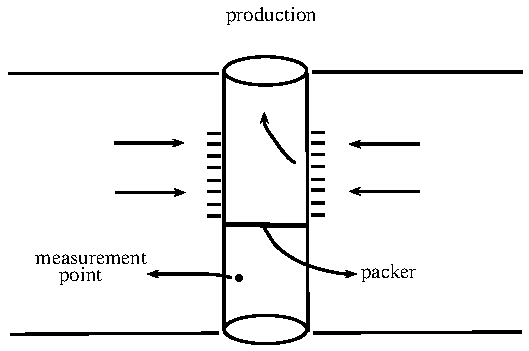
\includegraphics[scale=1]{Interference_test.pdf}
        \end{center}
        \caption{A schematic of a single well interference test.}
        \label{Interference_test}
    \end{figure}


    Multiple interference tests are run basically for the following two purposes,

    \begin{enumerate}[(1)]
        \item   to determine if there is hydraulic communication between wells.
        \item   quantify the inter-well formation properties, $k$ and $\phi c_{t}$
    \end{enumerate}

    \begin{figure}
        \begin{center}
        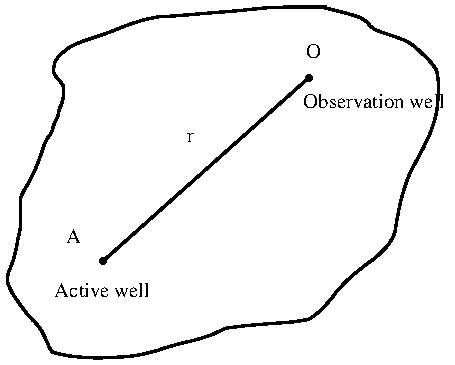
\includegraphics[scale=1]{Active_Obser_well.pdf}
        \end{center}
        \caption{Well \emph{A} is the active well and is where the production occurs. Well \emph{O} is the observation well where the pressure is measured.}
        \label{Active_Obser_well}
    \end{figure}

    The classical interference test procedure involves

    \begin{enumerate}[(i)]
        \item   shut in both wells and allow them to reach the \change[Murat \c{C}{\i}nar]{reservoir's average pressure}{average reservoir pressure, $p_{i}$ or $\overline{p}$}
        \item   produce well $A$ at a constant rate, q.
        \item   measure the pressure response in well $O$.
    \end{enumerate}

    If there is a measured response, then our first objective is achieved. \remove[Murat \c{C}{\i}nar]{To obtain }Inter-well values of $k$ and $\phi c_{t}$, \add[Murat \c{C}{\i}nar]{are obtained}\remove[Murat \c{C}{\i}nar]{the data analyzed} by semilog and TCA analysis techniques described earlier.

    \subsubsection{TCA procedure}

    \begin{enumerate}[(i)]
        \item   Overlay tracing paper (or transparency) on the type curve and plot the grid onto the tracing paper.
        \item   Plot all the data points.
        \item   Keeping the axes parallel move the $\Delta p$ versus $t$ graph with vertically and horizontally until the best match of $\Delta p$ versus $t$ with the type curve; i.e., $p_{D}$ versus $t_{D}/r{D}^{2}$ graph is obtained.
        \item   Pick the match point; [$(t)_{m}$,$(\Delta p)_{m}$] and [$(t_{D}/r_{D}^{2})_{m}$, $(p_{D})_{m}$]. It is convenient to use an intersection point of the grid on $\Delta p$ versus $t$ graph.
        \item   Calculate $k$ and $\phi c_{t}$ from Eqs. \ref{phct_match} and \ref{k_match_2} using the match point values.
        \item   Determine from $t_{D}/r_{D}^{2}>25$ criterion whether there are any data which will lie on a straight line on a plot of $\Delta p$ or ($p$) versus $lnt$ plot. If you determine that you will have such data, then proceed with the semilog analysis to determine $k$ and $\phi c_{t}$.
    \end{enumerate}

    \subsubsection{Use of derivative in TCA}
    Type curve analysis, before 1980, is based on the plotting $\Delta p$ versus $t$ and matching this data with the appropriate type curve (is a graphical representation of a theoretical model or interpretation model). After 1980, due primarily to Bourdet et al.'s work \cite{Bourdet_1983_1}, type curves incorporating the pressure derivatives (i.e.; $dp_{D}/dlnt_{D}$) become popular.
    Recall that for constant rate production, \remove[Murat \c{C}{\i}nar]{we have}

    \begin{equation*}
    {{p}_{D}}=\frac{2\pi kh\Delta p}{qB\mu }
    \end{equation*}

    and

    \begin{equation*}
    \frac{{{t}_{D}}}{r_{D}^{2}}=\frac{kt}{\phi {{c}_{t}}\mu {{r}^{2}}}
    \end{equation*}

    then
    \begin{equation*}
         \frac{{{t}_{D}}}{r_{D}^{2}}\frac{\partial {{p}_{D}}}{\partial {{{t}_{D}}}/{r_{D}^{2}}\;} =\frac{\partial {{p}_{D}}}{\partial \ln {{{t}_{D}}}/{r_{D}^{2}}\;}=\frac{\partial {{p}_{D}}}{\partial \ln {{t}_{D}}}=\frac{2\pi kh}{qB\mu }t\frac{\partial \Delta p}{\partial t}
    \end{equation*}

    \begin{equation}
     \frac{{{t}_{D}}}{r_{D}^{2}}\frac{\partial {{p}_{D}}}{\partial {{{t}_{D}}}/{r_{D}^{2}}\;}=\frac{2\pi kh}{qB\mu }\frac{\partial \Delta p}{\partial \ln t}
        \label{dpD_dtD_rD2}
    \end{equation}

    Eq. \ref{dpD_dtD_rD2} \add[Murat \c{C}{\i}nar]{when compared to} Eq. \ref{mD_no_p_var} \change[Murat \c{C}{\i}nar]{indicates}{reveals} that $\frac{\partial {{p}_{D}}}{\partial \ln {{t}_{D}}}$ is \change[Murat \c{C}{\i}nar]{made dimensionless}{non-dimensionalized} in the same way as $\Delta p$\remove[Murat \c{C}{\i}nar]{ is made dimensionless}. \change[Murat \c{C}{\i}nar]{This means that we can graph $p_{D}$ and $\frac{\partial {{p}_{D}}}{\partial {{{t}_{D}}}/{r_{D}^{2}}\;}$ on the same plot.}{Thus, $p_{D}$ and $\frac{\partial {{p}_{D}}}{\partial {{{t}_{D}}}/{r_{D}^{2}}\;}$ could be plotted on the same graph.} For the line source solution, \change[Murat \c{C}{\i}nar]{we}{one} can construct a type curve\remove[Murat \c{C}{\i}nar]{plot} that involves both $p_{D}$ versus $t_{D}/r_{D}^{2}$ and $\frac{\partial {{p}_{D}}}{\partial {{{t}_{D}}}/{r_{D}^{2}}\;}$ versus $t_{D}/r_{D}^{2}$  ,$p{{'}_{D}}={\partial {{p}_{D}}}/{\partial \ln {{t}_{D}}}$. Such a type curve is shown below for the line source solution - Fig. \ref{pD_pD_der_Line_Source}.


    \begin{figure}
        \begin{center}
        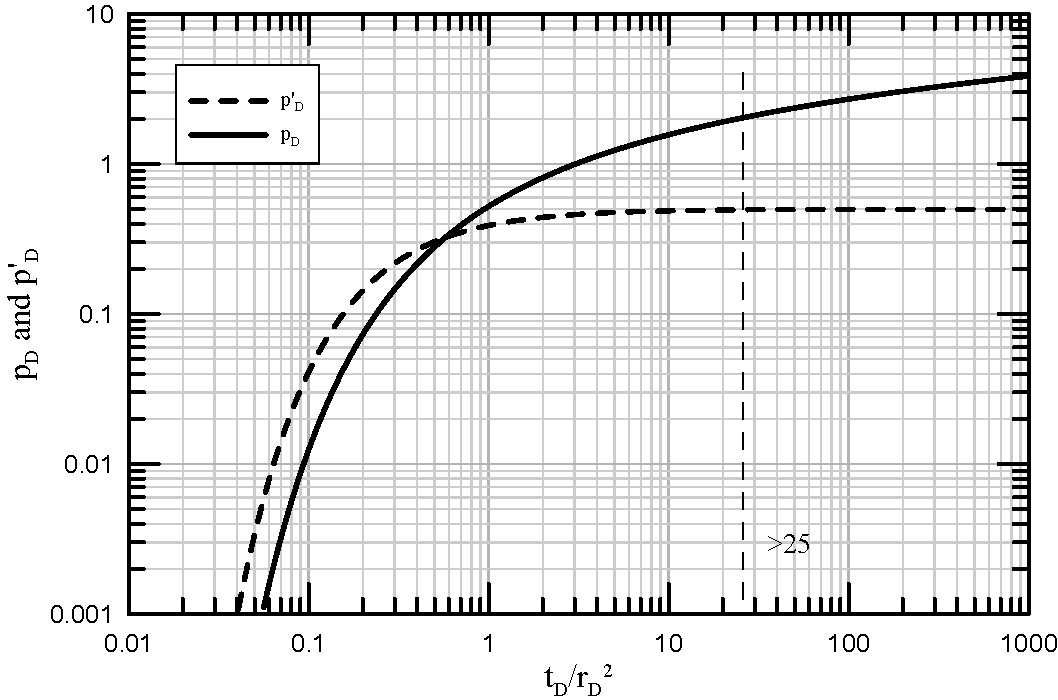
\includegraphics[scale=0.6]{pD_pD_der_Line_Source.pdf}
        \end{center}
        \caption{Line source solution.}
        \label{pD_pD_der_Line_Source}
    \end{figure}

    \change[Murat \c{C}{\i}nar]{To use derivative type curves, we match a plot of both $\Delta p$ and $\Delta p'$ versus $t$ simultaneously with the appropriate $p_{D}$ and $p_{D}'$ type curves. This should make type curve analysis more accurate because it requires both $\Delta p$ and $\Delta p'$ matched simultaneously.}{It is argued that using derivative type curves for type curve analysis is more accurate as it requires to match both both $\Delta p$ and $\Delta p'$ versus $t$ simultaneously with the appropriate $p_{D}$ and $p_{D}'$ type curves.} Since ${\partial {{p}_{D}}}/{\partial \ln {{t}_{D}}}$ is the instantaneous slope of $p_{D}$ plotted on a semilog \change[Murat \c{C}{\i}nar]{plot}{graph}, after $t_{D}/r_{D}^{2}>25$ $\frac{\partial {{p}_{D}}}{\partial {{{t}_{D}}}/{r_{D}^{2}}\;}$ should become constant and have a value of $1/2$. Similarly if the test data reach the time when the semilog approximation is applicable, ${\partial \Delta p}/{\partial \ln {{t}}}$ \change[Murat \c{C}{\i}nar]{should also become}{becomes} constant. In terms of type curve matching, this means that vertical match is fixed since the constant on flat portion of ${\partial \Delta p}/{\partial \ln {{t}}}$ should lie on the top of the constant portion of $\frac{\partial {{p}_{D}}}{\partial {{{t}_{D}}}/{r_{D}^{2}}\;}$. To complete the match, the test data only have to be moved in the horizontal direction until the rest of the $\Delta p$ and ${\partial \Delta p}/{\partial \ln {{t}}}$ data lie on the type curves.
    Another \change[Murat \c{C}{\i}nar]{alternative approach}{approach alternative} to derivative type curve matching has been proposed by Onur and Reynolds in 1988 \cite{Onur_1988_1}\change[Murat \c{C}{\i}nar]{. Such approach further simplified}{ simplifying} type curve matching procedure and \change[Murat \c{C}{\i}nar]{reduced}{reducing} non-uniqueness \add[Murat \c{C}{\i}nar]{the }problem (i.e., the data may seem to match the type curve equally well for different translation between the two sets of axes.).
    Onur and Reynolds proposed a derivative group based on a ratio of dimensionless pressure, $p_{D}$ to the pressure derivative, $p'_{D} = dp_{D}/d_lnt_{D}$; i.e.,

    \begin{equation}
        Rpp'=\frac{{{p}_{D}}}{2{{p}_{D}}'}=\frac{{{p}_{D}}}{2\left[ \frac{d{{p}_{D}}}{d\ln \left( {{{t}_{D}}}/{r_{D}^{2}}\; \right)} \right]}
        \label{Rpp_prime}
    \end{equation}

    to construct pressure derivative type curves. Since,

    \begin{equation*}
        {{p}_{D}}=\frac{2\pi kh\Delta p}{qB\mu }
    \end{equation*}
    and
    \begin{equation*}
    {{p}_{D}}=\frac{d{{p}_{D}}}{d\ln {{{t}_{D}}}/{r_{D}^{2}}\;}=\frac{2\pi kh}{qB\mu }\Delta p'
    \end{equation*}
    then

    \begin{equation}
        \frac{{{p}_{D}}}{2{{p}_{D}}'}=\frac{\Delta p}{2\Delta p'}
        \label{Rpp_prime_2}
    \end{equation}

    which indicates that the vertical scale of a plot ${{{p}_{D}}}/{\left( 2{{p}_{D}}' \right)}$ vs ${{{t}_{D}}}/{r_{D}^{2}}$ \change[Murat \c{C}{\i}nar]{will be}{is} identical to the vertical scale of a field data plot of $\frac{\Delta p}{2\Delta p'}$ versus $t$. Such a type curve is shown in Fig. \ref{Rpp} for the line source solution. Note that for the line source solution,

    \begin{equation}
    \frac{{{p}_{D}}}{2{{p}_{D}}'}=\frac{\Delta p}{2\Delta p'}=-\frac{1}{2}{Ei\left[ -\frac{r_{D}^{2}}{4{{t}_{D}}} \right]}/{\exp }\;\left[ -\frac{r_{D}^{2}}{4{{t}_{D}}} \right]
        \label{Rpp_prime_3}
    \end{equation}

    \begin{figure}
        \begin{center}
        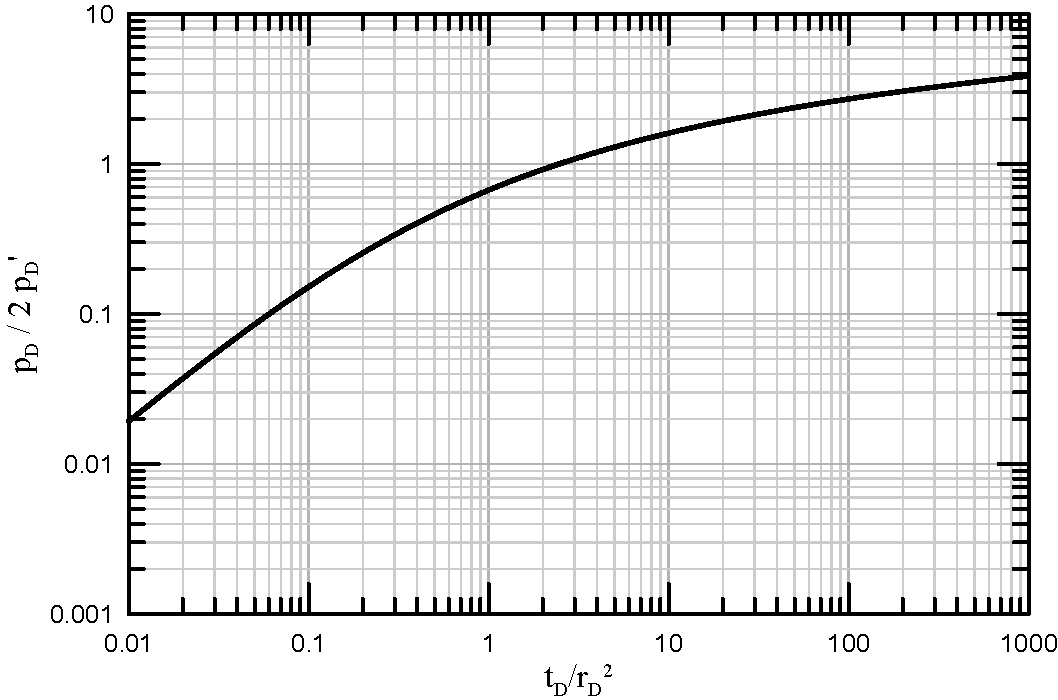
\includegraphics[scale=0.6]{Rpp.pdf}
        \end{center}
        \caption{Line source solution.}
        \label{Rpp}
    \end{figure}

    \textbf{Use of Rpp' type curve}

    \begin{enumerate}[(i)]
        \item   \change[Murat \c{C}{\i}nar]{In such a type curve, a}{A} match of ${\Delta p}/{2\Delta p'}$ versus $t$ data with the ${{{p}_{D}}}/{\left( 2{{p}_{D}}' \right)}$ type curve is obtained only by moving the field data plot in the horizontal direction. Once match is obtained, \remove[Murat \c{C}{\i}nar]{we determine the }time match point values\add[Murat \c{C}{\i}nar]{are determined}, [$t_{m}, (t_{D}/r_{D}^{2})_{m}$].
        \item   \change[Murat \c{C}{\i}nar]{Then, fixing}{Fix} the correspondence between time match point values, match the $\Delta p$ versus $t$ graph with $p_{D}$ versus ${{{t}_{D}}}/{r_{D}^{2}}$ graph only by the vertical movement. Once the match is obtained, \remove[Murat \c{C}{\i}nar]{we will determine }the pressure match point values \add[Murat \c{C}{\i}nar]{are determined}, [$(\Delta p)_{m}, (p_{D})_{m}$].
        \item   Since \remove[Murat \c{C}{\i}nar]{we determined }all match point values\change[Murat \c{C}{\i}nar]{we compute, then }{ are determined} $kh$ and $\phi c_{t}$ \add[Murat \c{C}{\i}nar]{are computed }from Eqs. \ref{phct_match} and \ref{k_match_2}.
    \end{enumerate}

    \change[Murat \c{C}{\i}nar]{If we have reached semilog straight line during the test, then}{If the semilog straight line is reached during the test, then}

    \begin{equation*}
    \begin{split}
    & \Delta p={{p}_{i}}-p\left( r,t \right)=\text{1}\text{.15129}\frac{qB\mu }{2\pi kh} \\
    & \left\{ \log \left( t \right)+\log \left[ \frac{kh}{\phi {{c}_{t}}\mu hr_{w}^{2}} \right]+\text{0}\text{.351378} \right\} \\
    \end{split}
    \end{equation*}

    and

    \begin{equation}
    \Delta p'=\frac{d\Delta p}{d\ln t}=\underbrace{\frac{\text{1}\text{.15129}}{2\pi \ln \left[ 10 \right]}}_{\text{0}\text{.0795773}}\frac{qB\mu }{kh}=\text{constant}
        \label{ddeltap_dlnt}
    \end{equation}

    Data in a time range where $\Delta p' = \text{constant}$ determines \change[Murat \c{C}{\i}nar]{that we have semilog data}{whether a semilog straight line is reached or not}. Alternatively, \change[Murat \c{C}{\i}nar]{during the test if we reached the semilog straight line then,}{if the semilog straight line is reached during the test then,}

    \begin{equation}
    \frac{\Delta p}{2\Delta p'}=\frac{{{p}_{D}}}{2{{p}_{D}}'}=\text{1}\text{.15129}\left\{ \begin{split}
    & \log \left( t \right)+ \\
    & \log \left[ \frac{kh}{\phi {{c}_{t}}\mu hr_{w}^{2}} \right]+\text{0}\text{.351378} \\
    \end{split} \right\}
        \label{Rpp_deltap}
    \end{equation}

    which indicates that a semilog plot of ${\Delta p}/{2\Delta p'}$ versus $t$ should yield a straight with a slope of $1.15129$ regardless of the values of the reservoir parameters, $k$, $h$, etc. Therefore, a semilog plot of ${\Delta p}/{2\Delta p'}$ versus $t$allow one to identify the time period (or periods) when the semilog straight line exists. Once such a plot identifies a semilog straight line, \change[Murat \c{C}{\i}nar]{we can employ semilog analysis with confidence}{semilog analysis is employed with confidence} (see Fig \ref{Rpp_Semilog}).

    \begin{figure}
        \begin{center}
        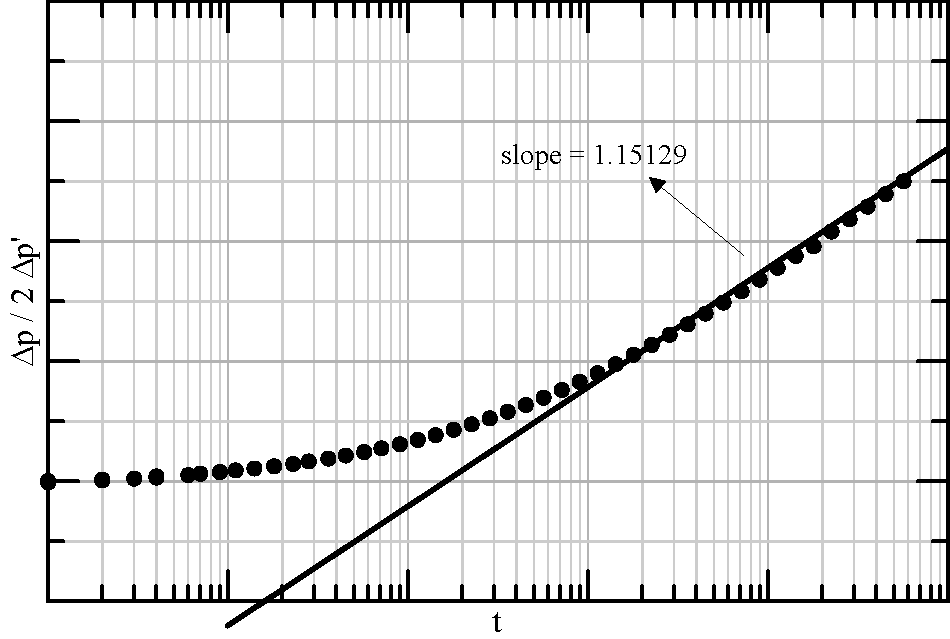
\includegraphics[scale=0.6]{Rpp_Semilog.pdf}
        \end{center}
        \caption{Rpp' semilog analysis.}
        \label{Rpp_Semilog}
    \end{figure}

    Although \remove[Murat \c{C}{\i}nar]{use of the }pressure derivatives \change[Murat \c{C}{\i}nar very]{is very}{are} useful in data analysis, it requires the computation of $\Delta p'$ versus $t$ by numerical differentiation. Resulting derivative data \add[Murat \c{C}{\i}nar]{is} often\remove[Murat \c{C}{\i}nar]{is} noisy to analyze properly with the derivative type curves. To eliminate this problem, \remove[Murat \c{C}{\i}nar]{recently some author's have proposed the }use of pressure integral functions \add[Murat \c{C}{\i}nar]{proposed}. \add[Murat \c{C}{\i}nar]{Unlike the derivative,} these functions help us to generate data essentially free of noise \remove[Murat \c{C}{\i}nar]{unlike the derivative. But these functions preserve}{ while preserving} the basic advantage of the pressure derivative (see Onur \cite{Onur_1989_2} and Blasingame \cite{Blasingame_1989_1}).

    \subsection{Formation Damage}
    Formation damage is a decrease in absolute permeability in the near wellbore region. Anything anything that causes a decrease in the permeability of the formations to hydrocarbons in the vicinity of wellbore will be referred to as true formation damage (invasion of drilling fluids, deposition of asphaltenes, or paraffins etc.). This will be associated with the skin factor (which is generally called true or mechanical skin factor).

    Skin factor arising from other than a change in permeability will be referred to as pseudo-skin factor. \change[Murat \c{C}{\i}nar]{Things that}{The following may} give rise to pseudo-skin factor \remove[Murat \c{C}{\i}]{are},

    \begin{enumerate}[(i)]
        \item   insufficient perforations
        \item   non-Darcy flow effect
        \item   restricted entry wells
        \item   multi-phase effects
    \end{enumerate}

    The formation damage is corrected by stimulation such as,

    \begin{enumerate}[(i)]
        \item   injecting acids to dissolve reservoir rock to increase $\phi$ and $k$.
        \item   injecting solvent to dissolve scale.
        \add[Murat \c{C}{\i}nar]{\item   injecting steam to dissolve contaminants and/or increase mobility.}
        \item   creating propped hydraulic fractures.
    \end{enumerate}

    "Skin effect" concept was introduced to the petroleum industry by van Everdingen \cite{Everdingen_1953_1} and Hurst \cite{Hurst_1953_1}. \change[Murat \c{C}{\i}nar very]{Both men did the following experiment.}{Now, we investigate the skin effect by following the steps below.} \Trcknote[Murat \c{C}{\i}nar very]{I had to make this change as I couldn't find the mentioned experiment in van Everdingen's paper.}
    
    \begin{enumerate}[(i)]
        \item   \change[Murat \c{C}{\i}nar]{Analyzed}{Analyze} a pressure test using basic semilog equation and \change[Murat \c{C}{\i}nar]{calculated}{calculate} a value for permeability knowing $\phi c){t} h$ and $\mu$. \Trcknote[Murat \c{C}{\i}nar]{I removed the semilog equation. It appears in the text many times.}
        \item   Using the values of $k$ and $\phi c_{t} h \mu$, \change[Murat \c{C}{\i}nar]{they computed}{compute} the theoretical pressures from the line source solution at $r=r_{w}$.
        \item   \change[Murat \c{C}{\i}nar]{They plotted}{Plot} the test data and the theoretical pressures on a semilog \change[Murat \c{C}{\i}nar]{plot}{graph}
    \end{enumerate}    
    
    \begin{figure}
        \begin{center}
        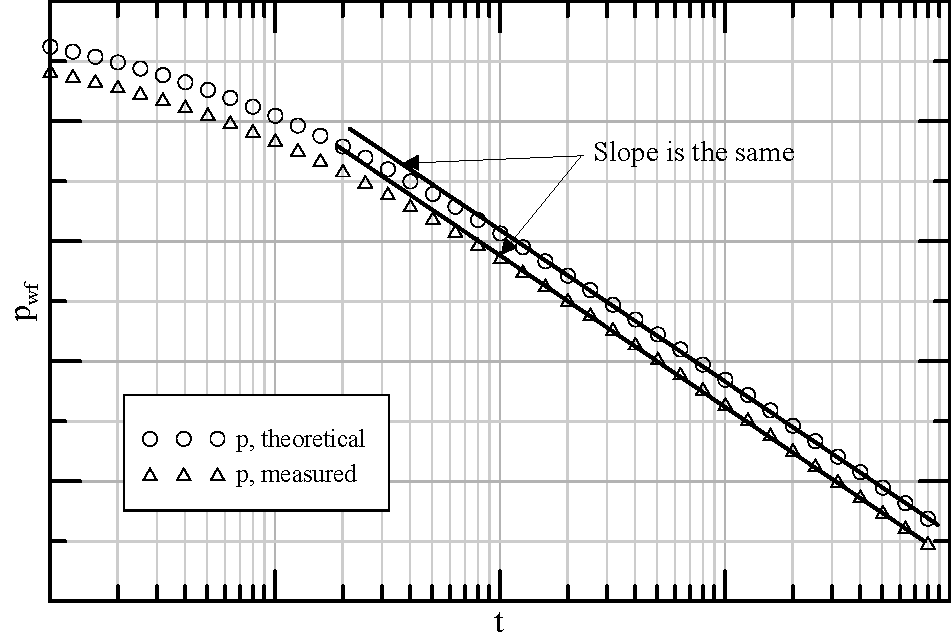
\includegraphics[scale=0.6]{Skin_effect.pdf}
        \end{center}
        \caption{Skin effect.}
        \label{Skin_effect}
    \end{figure}    
    
    \Trcknote[Murat \c{C}{\i}nar]{I added the following sentence}As Fig. \ref{Skin_effect} indicates, the theoretical curve is shifted with a constant value. \change[Murat \c{C}{\i}nar]{what they found out was that}{This is the same observation both van Everdingen and Hurst made} measured values of $p_{wf}$ were displaced below the theoretical straight line by a constant, i.e.;
    
    \begin{equation}
    \Delta {{p}_{measured}}=\Delta {{p}_{theoretical}}+\Delta {{p}_{skin}}
        \label{Skin}
    \end{equation}    
    
    when $\Delta {{p}_{skin}}$ is constant, van Everdingen and Hurst attributed the extra pressure drop to a low permeability region around the well. They called this region of altered permeability as the skin zone and \remove[Murat \c{C}{\i}nar]{called} the additional pressure drop due to the skin zone $\Delta {{p}_{skin}}$. They believed this low permeability region did not extend very far into the reservoir.
    
    \begin{figure}
        \begin{center}
        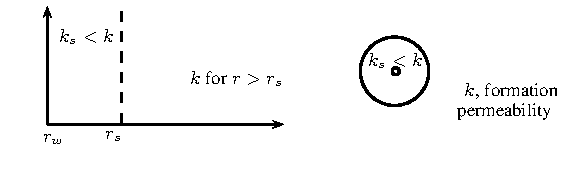
\includegraphics[scale=1.2]{Skin_1.pdf}
        \end{center}
        \caption{Skin zone.}
        \label{Skin_1}
    \end{figure}     
    
    \change[Murat \c{C}{\i}nar]{Let's}{Now} investigate the pressure profile due to an altered permeability for a constant rate production.
    
    \begin{figure}
        \begin{center}
        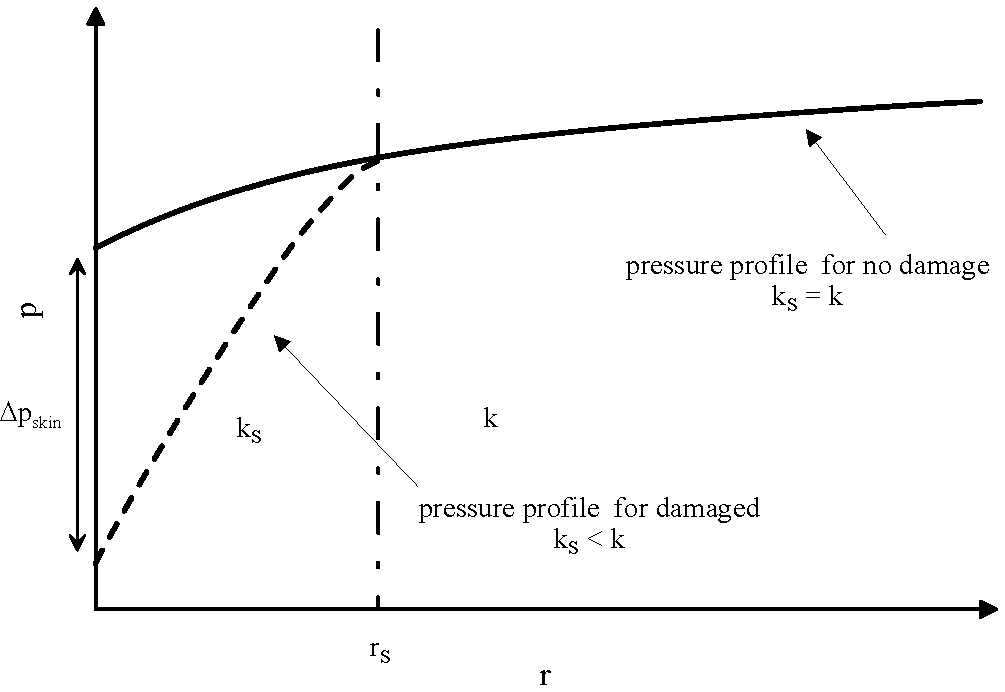
\includegraphics[scale=0.6]{Skin_effect_2.pdf}
        \end{center}
        \caption{Effect of skin on pressure profiles.}
        \label{Skin_effect_2}
    \end{figure}       
    
    Note that for a given flow rate, the lower permeability in the vicinity of the wellbore will cause an increase in the pressure drop.
    
    
    
    
    
    
    
    
    
    %\nomenclature[1]{$R$}{Ideal gas constant {$(8.314 J/gmol \cdot K)$}}%
    %\nomenclature{${\alpha }$}{Reaction order}%
    %\printnomenclature

    \bibliographystyle{plain}
    \bibliography{References}
%
\end{document}
